\documentclass{ieeeaccess}
\usepackage{cite}
\usepackage[hyphens]{url}
\Urlmuskip=0mu plus 1mu\relax
\usepackage{amsmath,amssymb,amsfonts}
\usepackage{algorithm}
\usepackage{algorithmic}
\usepackage{graphicx}
\usepackage{textcomp}
\usepackage{booktabs}
\usepackage{multirow}
\usepackage{amsthm}
\newtheorem{theorem}{Theorem}
\newtheorem{lemma}[theorem]{Lemma}
\newtheorem{corollary}[theorem]{Corollary}
\def\BibTeX{{\rm B\kern-.05em{\sc i\kern-.025em b}\kern-.08em
    T\kern-.1667em\lower.7ex\hbox{E}\kern-.125emX}}
\begin{document}
\history{Date of publication xxxx 00, 0000, date of current version xxxx 00, 0000.}
\doi{10.1109/TQE.2026.DOI}

\title{Advancing Quantum Graph Coloring: Custom State Preparation and MSB-Overflow Oracles for the Maximum Weight Colorable Subgraph Problem}
\author{\uppercase{Witchapat Issariyawat}\authorrefmark{1} and \uppercase{Kamonluk Suksen}\authorrefmark{1}}
\address[1]{Department of Computer Engineering, Chulalongkorn University, Bangkok, Thailand 10330 (e-mail: witchapat.iss@student.chula.ac.th; kamonluk@cp.eng.chula.ac.th)}

\corresp{Corresponding author: Witchapat Issariyawat (email: witchapat.iss@student.chula.ac.th).}

\begin{abstract}
Exact Grover oracles for the Maximum Weight Colorable Subgraph Problem (MWCSP) pay an $\mathcal{O}(S^2)$ Multi-Controlled X (MCX) cost at the comparator stage of every iteration, where $S$ is the weight-accumulator width. We propose an Overflow-Flag Range Comparator that replaces this comparator sub-block with a single CNOT: pre-loading the accumulator with the classical offset $\text{Offset} = 2^{S-1}-\text{Target}$ makes any configuration with score $\ge$ Target overflow into the Most Significant Bit, so the phase kickback reduces to one CNOT on the MSB. A Custom State Preparation layer adopting the Shukla--Vedula construction restricts the initial superposition to the $K^N$ valid colourings, removing the per-node invalid-colour checker subcircuits used by prior designs. On a like-for-like Qiskit pipeline against a reimplemented Belletti-style Boolean baseline, this combination saves $1$--$2$ qubits across our five benchmark topologies but pays $2.6\times$--$9.1\times$ more circuit depth, because the comparator-stage saving is recovered against a ripple-carry adder that the weighted formulation introduces and that now dominates the per-iteration cost. On a noise-free Aer simulator, a single complete Grover run at the empirically-optimal iteration count recovers the global optimum in $\ge 96\%$ of $2048$ shots across all five topologies, versus $3\%$--$22\%$ for QAOA at $p=7$ on the same shot budget. Resource projections through $N=100$ and a depolarising-noise sweep against IBM Heron-class baselines indicate that the resulting circuit depths sit beyond near-term NISQ coherence limits, so we position the design as a depth-prefactor reduction and a structural primitive for early fault-tolerant range-based combinatorial search rather than a near-term NISQ algorithm.
\end{abstract}

\begin{keywords}
Quantum Computing, Maximum Weight Graph Coloring, Grover's Algorithm, Space-Efficient Quantum Circuits, MSB Overflow Comparator, Fault-Tolerant Quantum Computing.
\end{keywords}

\titlepgskip=-15pt

\maketitle

\section{Introduction \& Related Work}
\label{sec:introduction}

\IEEEPARstart{T}{he} Graph $K$-Coloring problem is NP-complete and
arises in telecommunication frequency allocation, resource scheduling,
and compiler register optimization~\cite{west2001}. The Maximum Weight
Colorable Subgraph Problem (MWCSP) extends this formulation: given an
edge-weighted graph $G = (V, E, W)$, the objective is to find a color
assignment that maximizes the total weight of properly colored
(non-colliding) edges. Classical exact solvers become intractable as
$|V|$ and $|E|$ grow~\cite{garey1979}.

Quantum computing offers a quadratic speedup for combinatorial search
via amplitude amplification. However, near-term hardware imposes two
hard constraints: \emph{qubit width} (total available qubits) and
\emph{circuit depth} (gate layers before decoherence destroys the
quantum state). Exact digital quantum algorithms must therefore
minimize high-error-rate multi-qubit gates, particularly
Multi-Controlled X (MCX) and Toffoli (CCX) operations.

% -----------------------------------------------------------
\subsection{Limitations of QAOA}
% -----------------------------------------------------------

The Quantum Approximate Optimization Algorithm (QAOA) is the dominant
approach for quantum combinatorial optimization. It prepares a
parameterized ansatz by alternating a cost Hamiltonian $H_C$ and a
transverse-field mixer $H_M = \sum_{j=1}^{n_q} \sigma_x^{(j)}$:
%
\begin{equation}
|\psi_p(\boldsymbol{\gamma}, \boldsymbol{\beta})\rangle =
\prod_{k=1}^{p} e^{-i\beta_k H_M} e^{-i\gamma_k H_C}
|+\rangle^{\otimes n_q},
\end{equation}
%
where $p$ is the number of layers and $\boldsymbol{\gamma},
\boldsymbol{\beta}$ are classically optimized to maximize
$F_p = \langle\psi_p|H_C|\psi_p\rangle$.
For the MWCSP, $H_C$ encodes the graph such that its maximum
eigenvalue corresponds to the optimal coloring.

QAOA has two fundamental limitations. First, it provides no
exactness guarantee: convergence to the global optimum requires
$p \to \infty$, which is unachievable under finite coherence times.
Second, the classical parameter optimization is susceptible to barren
plateaus~\cite{mcclean2018barren}, where the gradient variance decays
as $\mathcal{O}(2^{-N})$ with system size, causing the optimizer to
stall for large graphs.

% -----------------------------------------------------------
\subsection{Overhead of Exact Grover Oracles}
% -----------------------------------------------------------

Grover's algorithm~\cite{grover1996, brassard2002} provides a
provable quadratic speedup and guarantees exact amplitude
amplification toward target states. The Grover iterator is:
%
\begin{equation}
G = -H^{\otimes n} U_0 H^{\otimes n} O,
\end{equation}
%
where $U_0 = 2|0\rangle\langle 0| - I$ and
$O = I - 2|x^*\rangle\langle x^*|$.
Applying $G$ for $\lfloor\frac{\pi}{4}\sqrt{M}\rfloor$ iterations
yields the target state with probability approaching $100\%$.

Applying Grover's algorithm to the MWCSP requires an arithmetic oracle
that accumulates edge weights and compares the total against a
threshold, all coherently in superposition. Standard comparators
implement an exact-match condition score $= T$ using MCX gates across
the full register width. Decomposing an $m$-qubit MCX under
nearest-neighbor connectivity requires $\mathcal{O}(m^2)$ two-qubit
gates per Grover iteration, creating a depth bottleneck. For dense
graphs, the ancilla count of existing exact-match oracles scales as
$\mathcal{O}((|V|+|E|)\log_2 K)$~\cite{belletti2025, glos2022,
clerc2023}, since each edge check requires dedicated indicator qubits
for every color $k \in K$ at every node.

\subsection{Quantum Arithmetic and Threshold Comparators}
\label{sec:qarith_related}
Our oracle inherits its arithmetic primitives from a mature line of work on quantum integer addition. Draper's QFT-based adder~\cite{draper2000} avoids ancillae by encoding the sum in Fourier phases; Cuccaro \textit{et al.}~\cite{cuccaro2004} introduced the linear-depth ripple-carry construction with a single ancilla that we use here; H\"aner, Roetteler, and Svore~\cite{haner2017factoring} showed how to perform in-place constant addition with dirty ancillae for Shor's algorithm; and Gidney~\cite{gidney2018halving} halved the $T$-count of addition by replacing each Toffoli with a temporary logical-AND gadget. Composing these adders with the rest of the toolbox~\cite{haner2018arithmetic,montanaro2016} gives a standard recipe for evaluating ``\,$\sigma \ge T$\,'' on a quantum register: subtract $T$ in place and read the carry-out (equivalently, the most-significant bit of the two's-complement difference). The subtract-and-test pattern is folklore in the modular-arithmetic literature and is implicit in Shor's modular reduction~\cite{haner2017factoring}.

The MSB-Overflow oracle introduced in this paper differs from that folklore pattern in one specific way that matters for Grover search. Rather than executing a quantum subtraction of $T$ in every iteration, we precompute $\mathrm{Offset} = 2^{S-1} - T$ \emph{classically} and impose it on the accumulator with a layer of single-qubit $X$ gates at the start of the iteration. The accumulator is left unsigned: the per-iteration cost is the layer of $X$ gates (no Toffolis) plus the additions of $w_e$ for valid edges, and the threshold test reduces to one CNOT controlled by the MSB. Compared to a subtract-then-test implementation that places a full ripple-carry comparator on the critical path, this saves an $\mathcal{O}(S)$-depth Toffoli block per iteration, which is the regime where Grover's amplitude amplification multiplies the per-iteration cost $R = \lfloor(\pi/4)\sqrt{M/|\mathcal{S}^*|}\rfloor$ times (Section~\ref{sec:practical_limits}). Section~\ref{sec:formal_proofs} establishes the soundness of this transformation; the saving is what justifies presenting it as a primitive of independent interest rather than merely an implementation detail of MWCSP.

% -----------------------------------------------------------
\subsection{Belletti's Unweighted Baseline}
% -----------------------------------------------------------

Belletti \textit{et al.}~\cite{belletti2025} formalized a
Grover-based oracle for unweighted Graph $K$-Coloring. Their design
initializes all node registers with Hadamard gates, producing a
uniform superposition over $2^{Nq}$ states. When $K$ is not a power
of 2 (e.g., $K=3$ requires $q=2$ qubits, introducing the invalid
state $|11\rangle$), dedicated invalid-color checker subcircuits must
suppress these phantom states at every node, increasing both qubit
width and MCX depth.

Their scope is strictly the unweighted K-Coloring decision
problem: throughout the paper the cost metric is whether the
coloring is proper, and no edge or vertex weights are ever
introduced (see~\cite[Sec.~III]{belletti2025} for the oracle
definition and \cite[Table~I]{belletti2025} for the asymptotic
complexity, both of which depend only on $N$, $K$, and the edge
count, never on weights). Consistent with this Boolean framing,
the phase-marking step is implemented by an MCX over the ancillae
that hold the per-edge equality and per-node validity flags
(\cite[Sec.~III.C]{belletti2025}), so it triggers only on
configurations for which every comparator simultaneously evaluates
to $|1\rangle$. On a frustrated input where no proper $K$-coloring
exists, that conjunction is unsatisfiable and the oracle marks
no states, leaving the post-diffusion distribution uniform.

% -----------------------------------------------------------
\subsection{Proposed Architecture}
% -----------------------------------------------------------

Belletti's design has two limitations that prevent direct extension to
the MWCSP: (1) it cannot accumulate edge weights, and (2) it returns
no solution on frustrated graphs. We address both with two changes.

\textbf{Custom State Preparation.} We replace the Hadamard
initialization with an operator $\mathcal{A}_\mathrm{init}$ that
produces a uniform superposition over exactly the $K^N$ valid
colorings. This eliminates phantom states and the associated
invalid-color checkers, reducing both qubit width and oracle depth.

\textbf{MSB-Overflow Comparator.} We replace the exact-match MCX
comparator with a carry-ripple weight accumulator and an
MSB-overflow flag. Initializing the accumulator with a classical
offset $\mathrm{Offset} = 2^{S-1} - T$ causes any coloring with
score $\geq T$ to overflow the register and flip the MSB. The
phase-kickback then requires only a single CNOT on the MSB,
reducing comparator depth from $\mathcal{O}(S^2)$ to
$\mathcal{O}(1)$.

% -----------------------------------------------------------
\subsection{Contributions}
% -----------------------------------------------------------

This paper proposes a space-efficient Grover oracle family for the
MWCSP with the following contributions:
%
\begin{enumerate}
    \item \emph{Integration of the Shukla--Vedula uniform-superposition
    construction~\cite{shukla2024} as a Custom State Preparation layer
    within a Grover oracle for arbitrary $K$.} The component itself is
    not new, but using it to remove the per-node invalid-colour
    checker subcircuits (and the MCX depth they impose every iteration)
    is, to our knowledge, not previously documented in the MWCSP
    literature (Section~\ref{sec:methodology}).

    \item \emph{An MSB-Overflow Range Comparator obtained by relocating
    the threshold subtraction from the quantum circuit to a classical
    offset.} Subtract-and-test threshold comparators are folklore in
    the quantum-arithmetic literature
    (Section~\ref{sec:qarith_related}); our specific variant
    pre-computes $\mathrm{Offset} = 2^{S-1} - T$ classically and loads
    it with a single layer of $X$ gates, so the quantum critical path
    contains no in-place subtraction and the threshold readout reduces
    to one CNOT on the MSB. Section~\ref{sec:formal_proofs}
    establishes soundness on the discrete accumulator domain.

    \item \emph{Three oracle variants---Min Width, Min Depth, and
    Balanced---that span the width--depth continuum,} with the
    Balanced chunk size set by the parameter-free heuristic of
    Belletti~\textit{et al.}~\cite{belletti2025}. We measure all three
    on the same Qiskit pipeline and report the actual depth gap
    between Min Width and Min Depth ($1$--$11\%$ at $N \le 12$),
    isolating the ripple-carry adder as the remaining serialisation
    bottleneck (Section~\ref{sec:methodology}).

    \item \emph{A like-for-like resource benchmark against two
    baselines.} We reimplement the Belletti~\cite{belletti2025}
    Boolean oracle and a one-hot QAOA ($p{=}7$, multi-restart L-BFGS-B)
    in the same Qiskit pipeline, reporting transpiled gate counts,
    per-iteration depths, empirical $96$--$99\%$ Grover success rates
    versus QAOA $3$--$22\%$, and a noise sweep against IBM Heron-class
    depolarising parameters (Section~\ref{sec:benchmarks}).
\end{enumerate}

\section{Problem Formulation \& Cost Function}
\label{sec:formulation}

\subsection{Mathematical Model of the MWCSP}

We model the instance as an undirected, edge-weighted graph $G = (V, E, W)$. The vertex set $V = \{v_1, \dots, v_n\}$ holds the nodes to be coloured, $E \subseteq V \times V$ holds the edges encoding pairwise constraints, and each edge $(u, v) \in E$ carries a positive integer weight $w_{(u,v)} \in \mathbb{Z}^+$.

A valid coloring is a map $C: V \to \{0, 1, \dots, K-1\}$. The standard unweighted $K$-coloring problem asks whether a $C$ exists with $C(u) \neq C(v)$ for every $(u,v) \in E$; on dense or low-$K$ instances (e.g.\ $K_4$ with $K=3$) no such $C$ exists. The MWCSP relaxes this to a maximisation problem: among all colorings, find one that maximises the total weight of properly coloured edges. Formally,
\begin{equation}
\text{Maximize: } \text{Score} = \sum_{(u, v) \in E} w_{(u,v)} \cdot \Delta_{(u,v)},
\end{equation}
where $\Delta_{(u,v)} = 1$ if $C(u) \neq C(v)$ and $0$ otherwise.

\subsection{Translating the Objective to a Hamiltonian}
\textit{Scope clarification:} The Hamiltonian formulation below is presented solely for theoretical completeness and to establish a direct connection with the QAOA literature reviewed in Section~\ref{sec:introduction}. Our proposed oracle architecture (Section~\ref{sec:methodology}) operates entirely as a digital arithmetic circuit and does \textbf{not} rely on Hamiltonian time-evolution or variational parameter optimization. Nevertheless, casting the MWCSP objective as a Cost Hamiltonian $H_C$ is valuable because it (i) exposes the eigenvalue spectrum whose maximum eigenstate our Grover oracle targets, and (ii) enables direct structural comparison with QAOA-based approaches in Section~V.

For a binary domain ($K=2$), the classical objective maps directly to the Ising Hamiltonian:
\begin{equation}
H_C = \sum_{(u,v) \in E} w_{(u,v)} \frac{I - \sigma_z^{(u)} \sigma_z^{(v)}}{2},
\end{equation}
whose largest eigenvalue of the diagonal $2^N \times 2^N$ matrix encodes the maximum-weight colourable subgraph. For $K > 2$ the binary encoding allocates $q = \lceil \log_2(K) \rceil$ qubits per node, and the inequality $C(u) \neq C(v)$ becomes a bitwise comparison across the two $q$-qubit registers, producing $H_C$ terms with up to $2q$-body Pauli-$Z$ interactions:
\begin{equation}
\mathbb{1}[C(u) \neq C(v)] = I - \prod_{i=0}^{q-1} \frac{I + \sigma_z^{(u,i)} \sigma_z^{(v,i)}}{2},
\label{eq:high_body}
\end{equation}
which expands into $\sigma_z$ products of order up to $2q$ (e.g.\ $4$-body for $K \in \{3,4\}$, $6$-body for $K \in \{5,\dots,8\}$). Because superconducting hardware natively realises only $1$- and $2$-body Pauli interactions, evolving under this $H_C$ requires Trotter decomposition into deep entangling layers or quadratization gadgets with auxiliary qubits. This is the structural reason QAOA implementations fall back to one-hot encoding (Section~\ref{sec:comparison}); our oracle sidesteps the issue entirely because it never evolves under $H_C$ and instead evaluates $\mathbb{1}[C(u) \neq C(v)]$ via explicit Boolean logic in the computational basis (Section~\ref{sec:methodology}).

\subsection{Binary Quantum Encoding Limitations \& Amplitude Leakage}

We encode the colour of each node in a register of $q = \lceil \log_2(K) \rceil$ qubits, following the standard binary encoding of~\cite{saha2020}. Writing $|c\rangle = |q_{q-1} \dots q_0\rangle \in \{0,1\}^q$ for a single-node register, the standard Hadamard initialisation $H^{\otimes Nq}$ produces the uniform superposition over $2^{Nq}$ basis states with amplitude $1/\sqrt{2^{Nq}}$ each.

When $K$ is not a power of $2$, this initialisation overshoots the valid colour set. For $K = 3$ at $q = 2$, the phantom state $|11\rangle$---which would correspond to colour value $3$, outside the valid range $\{0,1,2\}$---appears in the global superposition with the same amplitude as the valid colours.

The leakage compounds across nodes: $M_{\text{total}} = 2^{Nq}$ exceeds the valid target space $M_{\text{valid}} = K^N$ by a factor of $(2^q/K)^N$; at $K = 3$ and $N = 12$, more than $99\%$ of the initial amplitude sits on phantom configurations. Grover amplification therefore spends iterations on states that are infeasible by construction. Our custom state preparation eliminates this by restricting the initial superposition to the valid $K^N$ subspace before any arithmetic step (Section~\ref{sec:methodology}).

\subsection{Background: Quantum Carry-Ripple Arithmetic}
To accumulate integer weights inside the superposition without measurement, the oracle must perform arithmetic in place. The Quantum Carry-Ripple Adder of Cuccaro \textit{et al.}~\cite{cuccaro2004} accomplishes this with cascaded MCX/CCX gates, computing both the bitwise sum and a carry bit that propagates from LSB to MSB. At the logical level the carry chain imposes a depth of $\mathcal{O}(n)$ Toffoli layers, which is what we will refer to as $D_{\mathrm{adder}}$ in the variant analysis of Section~\ref{sec:methodology}. After transpilation to the hardware-native $\{CX, RZ, SX, X\}$ basis without borrowed ancillae, however, every Toffoli expands by an $\mathcal{O}(n)$ factor under nearest-neighbor connectivity~\cite{barenco1995,nielsen2010}, so a single addition compiles to $\mathcal{O}(S^2)$ two-qubit layers in practice (where $S$ is the accumulator width including the MSB flag). The in-place property and single-ancilla footprint of the ripple-carry construction are what we exchange this depth penalty for: replacing it with carry-save or partial-sum-tree adders~\cite{thapliyal2010} would lower the transpiled depth to $\mathcal{O}(S \log S)$ but cost additional ancillae, an avenue we leave to future work.

\section{Proposed Methodology}
\label{sec:methodology}

\subsection{Custom Initialization Geometry}
Before the arithmetic stage, the oracle must prepare a superposition over only the $K^N$ valid colourings. The Hadamard initialisation $H^{\otimes Nq}$ used by~\cite{belletti2025} populates the larger $2^{Nq}$ space and therefore requires per-node invalid-colour checker subcircuits to suppress the phantom states. We replace this with the Shukla--Vedula uniform-superposition construction~\cite{shukla2024}, which uses $R_y$ rotations and controlled-Hadamards to produce uniform amplitude over $|0\rangle, \dots, |K-1\rangle$ with zero amplitude on $|K\rangle, \dots, |2^q-1\rangle$. Integrating this operator as $\mathcal{A}_\mathrm{init}$ removes the invalid-colour checkers and the MCX depth they would impose on every Grover iteration.

$\mathcal{A}_{\text{init}}$ is a unitary on each $q$-qubit register:
\begin{equation}
\mathcal{A}_{\text{init}} |0\rangle^{\otimes q} = \frac{1}{\sqrt{K}} \sum_{c=0}^{K-1} |c\rangle
\end{equation}
Applied across all $N$ vertices, the global initial state becomes
\begin{equation}
|\Psi_{\text{initial}}\rangle = \bigotimes_{u \in V} \mathcal{A}_{\text{init}} |0\rangle_u = \frac{1}{\sqrt{K^N}} \sum_{X \in \mathcal{V}} |X\rangle \label{eq:initial}
\end{equation}
where $\mathcal{V} = \{0, \dots, K-1\}^N$. For $K$ not a power of $2$, this construction sidesteps the per-node invalid-colour checks at every Grover iteration, leaving those ancillas available for the weight accumulator.

\paragraph{Generalized Construction for Arbitrary $K$}
While Fig.~\ref{fig:circuit_sp} illustrates the $K=3$ case, the construction generalizes to any $K \ge 2$ via a recursive balanced partitioning strategy. For $q = \lceil \log_2(K) \rceil$ qubits, the operator $\mathcal{A}_{\mathrm{init}}^{(K)}$ is built recursively as follows:

\textit{General rotation angle.} At each recursion level, the MSB qubit receives an $R_y$ rotation with angle:
\begin{equation}
\theta = 2\arccos\!\left(\sqrt{\frac{\lceil K/2 \rceil}{K}}\right)
\label{eq:ry_general}
\end{equation}
which allocates probability $\lceil K/2 \rceil / K$ to the MSB$=|0\rangle$ branch and $\lfloor K/2 \rfloor / K$ to the MSB$=|1\rangle$ branch. When $K$ is a power of 2, this reduces to $\theta = \pi/2$ (i.e., a Hadamard), recovering the standard $H^{\otimes q}$ construction as a special case.

The explicit construction procedure is formalized in Algorithm~\ref{alg:ainit}.

\begin{algorithm}[h!]
\caption{Generalized $\mathcal{A}_{\mathrm{init}}^{(K)}$ Construction}\label{alg:ainit}
\begin{algorithmic}[1]
\REQUIRE Color count $K \ge 2$, qubit register $[q_{q-1}, \dots, q_0]$
\IF{$K = 1$}
    \STATE \textbf{return} (identity; no gates needed)
\ELSIF{$K = 2^m$ for some integer $m$}
    \STATE Apply $H^{\otimes m}$ to qubits $[q_{m-1}, \dots, q_0]$
\ELSE
    \STATE $K_L \leftarrow \lceil K/2 \rceil$,\quad $K_U \leftarrow \lfloor K/2 \rfloor$
    \STATE Apply $R_y(\theta)$ on $q_{q-1}$ with $\theta$ from Eq.~\eqref{eq:ry_general}
    \STATE Controlled on $q_{q-1} = |0\rangle$: recursively apply $\mathcal{A}_{\mathrm{init}}^{(K_L)}$ on $[q_{q-2}, \dots, q_0]$
    \STATE Controlled on $q_{q-1} = |1\rangle$: recursively apply $\mathcal{A}_{\mathrm{init}}^{(K_U)}$ on $[q_{q-2}, \dots, q_0]$
\ENDIF
\end{algorithmic}
\end{algorithm}

\textit{Gate count analysis.} Each recursion level contributes at most one $R_y$ gate and one controlled gate (CH or controlled-$R_y$). Since the recursion depth is bounded by $q = \lceil \log_2(K) \rceil$, the total gate count per node is $\mathcal{O}(q)$---i.e., $\mathcal{O}(\log K)$. For common cases: $K=2$ requires 1 $H$ gate, $K=3$ requires 1 $R_y$ + 1 CH = 2 gates, $K=4$ requires 2 $H$ gates, and $K=5$ requires 1 $R_y$ + 1 CH + 1 $R_y$ = 3 gates. This sub-linear scaling ensures that the state preparation overhead remains negligible relative to the oracle body even for large color counts.

\subsection{Space-Efficient Weight Accumulation via Phase Shifting}
For each individual edge $(u,v) \in E$ maintaining a static predefined topological weight $w$, the oracle employs a localized binary hardware comparator to verify if the corresponding nodes maintain distinct colors ($C(u) \neq C(v)$). If the geometric topological condition is confirmed valid, the weight $w$ must be mathematically accumulated into the global score tracking register.

Rather than storing $w$ in a dedicated quantum register---which would double the accumulator's qubit footprint---we embed $w$ classically inside a shifted power-of-2 adder. The accumulation phase composes cascaded ripple-carry networks~\cite{nielsen2010} parameterised by the classical bit pattern of $w$.

Adding the classical integer $w$ to the accumulator $|s\rangle$ thus reduces to a sequence of MCX-based increments at the bit positions where $w$ has a $1$, each controlled by the single edge-validity ancilla $|ans\rangle$. This removes the need for any quantum multiplier or weight register: every edge contributes only an in-place increment chain.

\subsection{The Overflow-Flag Phase Comparator: A Depth Resolution}
The primary bottleneck preventing exact Grover search from being executed on numeric optimization problems is the depth of the terminating phase-kickback validation.

\paragraph{The Baseline Constraint Overhead}
Traditional Grover formulations for numerical optimization compute exact magnitude equality. To verify that the score register $S$ has reached a target $T$, the standard approach implements a binary condition $\text{score} = T$, which requires Multi-Controlled X (MCX) gates spanning the full register width.

Two baselines exist for this comparator step, and their costs differ. (i) Decomposing an $m$-qubit MCX into a $\{CX, U_3\}$ basis under nearest-neighbor connectivity, without borrowed ancillae, requires $\mathcal{O}(m^2)$ two-qubit gates~\cite{barenco1995,nielsen2010}; this is the cost paid by oracles that read the equality condition off the full register through one large MCX. (ii) Alternative \emph{ripple-carry} comparators that subtract $T$ in place and read the carry-out~\cite{thapliyal2010,oliveira2007} achieve $\mathcal{O}(S)$ depth at the cost of one extra ancilla and a full ripple-carry subtractor on the critical path of every Grover iteration. Identifying configurations where $\text{score} \ge T$ (i.e., range rather than equality) does not change these scalings, but in both cases the comparator sits on the critical path and is multiplied by the Grover repetition count $R$.

\paragraph{Our $\mathcal{O}(1)$-Gate Algorithm}
To bypass this bottleneck, we extend the score register by one qubit, designating it the Most Significant Bit (MSB). Rather than evaluating magnitude post-addition, we initialize the accumulator with a classically pre-computed offset:
\begin{equation}
\text{Offset} = 2^{S-1} - \text{Target}
\end{equation}
where $S = \lceil \log_2(W_{\max} + 1) \rceil + 1$ is the total accumulator width including the MSB flag.

The Offset is encoded into the zero-state basis by a single layer of Pauli-X gates applied to the positions where the binary representation of Offset has a 1. As the controlled adders accumulate valid edge weights $w$ during oracle execution, any configuration whose score reaches the Target overflows the lower $S{-}1$ data qubits, flipping the MSB from $|0\rangle$ to $|1\rangle$.

Consequently, the oracle phase inversion $S_f = I - 2|\text{score} \ge T\rangle\langle\text{score} \ge T|$ reduces from an $S$-qubit MCX (or an $\mathcal{O}(S)$-depth ripple-carry comparator) to a single CNOT applied to the MSB flag, shrinking the per-iteration comparator depth to $\mathcal{O}(1)$ as illustrated in Fig.~\ref{fig:circuit_overflow}. Relative to the MCX baseline above (i), the saving is $\mathcal{O}(S^2) \to \mathcal{O}(1)$; relative to the ripple-carry baseline (ii), it is $\mathcal{O}(S) \to \mathcal{O}(1)$. In both cases the elimination is from the critical path, so the per-iteration saving is multiplied by $R$. This construction is related to but distinct from the standard subtract-and-test-carry comparator used in quantum modular arithmetic (Section~\ref{sec:qarith_related}): the threshold subtraction is absorbed into a classical $\mathrm{Offset}$ that is loaded with $X$ gates only, eliminating the per-iteration ripple-carry subtractor from the critical path.

\begin{algorithm}[h!]
\caption{Continuous MSB-Overflow Oracle Synthesis}\label{alg:oracle}
\begin{algorithmic}[1]
\REQUIRE Graph $G=(V,E,W)$, Target Weight $T$
\STATE \textbf{Initialize:} $N \leftarrow |V|$, $S \leftarrow \lceil \log_2(W_{\max} + 1) \rceil + 1$
\STATE \textbf{Classical Pre-compute:} $\text{Offset} \leftarrow 2^{S-1} - T$
\STATE Apply $\mathcal{A}_{\text{init}}$ to all node registers
    \COMMENT{Prune $|v\rangle \notin K^N$; no phantom states remain}
\FOR{$i = 0$ to $S-2$}
    \IF{$\text{bit}(i,\, \text{Offset}) = 1$}
        \STATE Apply $X$ to accumulator qubit $s_i$
            \COMMENT{Encode classical offset into zero-state basis}
    \ENDIF
\ENDFOR
\FOR{each edge $e = (u,v) \in E$}
    \STATE \COMMENT{\textit{Stage A --- Quantum Collision Detection}}
    \STATE Compute $|{ans}_e\rangle \leftarrow \textsc{CollisionCheck}(|u\rangle,\,|v\rangle)$
        \COMMENT{CX-X-MCX sequence; $|{ans}_e\rangle\!=\!|1\rangle$ iff $C(u)\!\neq\! C(v)$;
                 no measurement performed --- $|{ans}_e\rangle$ remains entangled in superposition}
    \STATE \COMMENT{\textit{Stage B --- Coherent Controlled Addition}}
    \STATE Apply $\textsc{Controlled-Add}(w_e)$ to accumulator,
           controlled on $|{ans}_e\rangle = |1\rangle$
        \COMMENT{Addition executes coherently across all superposition branches simultaneously}
    \STATE \COMMENT{\textit{Stage C --- Uncompute Ancilla}}
    \STATE Apply $\textsc{CollisionCheck}^{\dagger}(|u\rangle,\,|v\rangle)$
           to restore $|{ans}_e\rangle \rightarrow |0\rangle$
        \COMMENT{Required to disentangle ancilla; prevents decoherence of score register}
\ENDFOR
\STATE \textbf{Phase Trigger:}
       Apply $CNOT$ with control $s_{S-1}$ (MSB flag), target $|\text{phase}\rangle$
    \COMMENT{MSB $= |1\rangle$ if accumulated score $\geq T$;
             triggers global phase kickback $-1$ exclusively on target states}
\STATE Apply inverse of steps 4--13 to restore accumulator to $|\text{Offset}\rangle$
    \COMMENT{Uncomputes all Carry-Ripple Adders and $X$ gates}
\end{algorithmic}
\end{algorithm}


\subsection{Formal Correctness Analysis}
\label{sec:formal_proofs}

We now rigorously establish the mathematical foundations underpinning the MSB-Overflow mechanism. The following results prove that the overflow-flag detection is both \textit{sound} (no false positives) and \textit{complete} (no false negatives) for arbitrary graph topologies and color counts.

\begin{theorem}[MSB Overflow Correctness]
\label{thm:overflow}
Let $\mathcal{R}$ be an $S$-bit quantum accumulator register whose individual qubits are denoted $s_0, s_1, \dots, s_{S-1}$, indexed from the Least Significant Bit ($s_0$) to the Most Significant Bit ($s_{S-1}$). Let $S = \lceil \log_2(W_{\max} + 1) \rceil + 1$, where $W_{\max} = \sum_{(u,v) \in E} w_{(u,v)}$ is the maximum achievable score. Suppose the register is initialized to the classical value $\mathrm{Offset} = 2^{S-1} - \mathrm{Target}$, where $0 \le \mathrm{Target} \le W_{\max}$. After accumulating a non-negative integer score $\sigma \in [0, W_{\max}]$ via modular carry-ripple addition, the MSB flag qubit $s_{S-1}$ satisfies:
\[
s_{S-1} = |1\rangle \quad \Longleftrightarrow \quad \sigma \ge \mathrm{Target}.
\]
\end{theorem}

\begin{proof}
After accumulation, the register value (interpreted as an unsigned $S$-bit integer) is
\[
R = \mathrm{Offset} + \sigma = (2^{S-1} - \mathrm{Target}) + \sigma.
\]

\textit{No overflow wrap-around.} We first verify that $R < 2^S$ for all valid $\sigma$. By the sizing constraint, $S \ge \lceil \log_2(W_{\max} + 1) \rceil + 1$, so $2^{S-1} \ge W_{\max} + 1$. Therefore:
\[
R \le (2^{S-1} - 0) + W_{\max} = 2^{S-1} + W_{\max} < 2^{S-1} + 2^{S-1} = 2^S.
\]
Thus the addition never wraps around modulo $2^S$, and $R$ is exact.

\textit{Forward direction ($\sigma \ge \mathrm{Target} \Rightarrow s_{S-1} = |1\rangle$).} If $\sigma \ge \mathrm{Target}$, then $R = 2^{S-1} + (\sigma - \mathrm{Target}) \ge 2^{S-1}$. In binary, any value $\ge 2^{S-1}$ has its $(S{-}1)$-th bit set to $1$.

\textit{Reverse direction ($s_{S-1} = |1\rangle \Rightarrow \sigma \ge \mathrm{Target}$).} If $s_{S-1} = |1\rangle$, then $R \ge 2^{S-1}$, which gives $\sigma \ge \mathrm{Target}$.


\textit{Edge cases.}
\begin{enumerate}
    \item[(i)] $\sigma = \mathrm{Target}$: $R = 2^{S-1}$ exactly, whose binary form is $1\underbrace{00\cdots0}_{S-1}$, so $s_{S-1} = |1\rangle$. \textit{The boundary score is correctly accepted.}
    \item[(ii)] $\sigma = \mathrm{Target} - 1$: $R = 2^{S-1} - 1$, whose binary form is $0\underbrace{11\cdots1}_{S-1}$, so $s_{S-1} = |0\rangle$. \textit{One point below the boundary is correctly rejected.}
    \item[(iii)] $\sigma = 0$: $R = 2^{S-1} - \mathrm{Target} < 2^{S-1}$ (since $\mathrm{Target} \ge 1$ for non-trivial instances), so $s_{S-1} = |0\rangle$. \textit{The zero-score case is correctly rejected.}
    \item[(iv)] $\sigma = W_{\max}$: $R < 2^S$ as shown above, so the register does not wrap around and the result is well-defined. \textit{The maximum-score case remains within representable range.}
\end{enumerate}
\end{proof}

\begin{lemma}[Custom State Preparation Correctness]
\label{lem:state_prep}
For any integer $K \ge 2$ with $q = \lceil \log_2(K) \rceil$ qubits per node, there exists a unitary operator $\mathcal{A}_{\mathrm{init}}$---constructed via the deterministic balanced-partitioning scheme of Shukla and Vedula \cite{shukla2024}---decomposable into $\mathcal{O}(q)$ single-qubit $R_y$ rotations and at most $q - 1$ controlled gates, requiring no ancilla qubits, such that:
\[
\mathcal{A}_{\mathrm{init}} |0\rangle^{\otimes q} = \frac{1}{\sqrt{K}} \sum_{c=0}^{K-1} |c\rangle,
\]
with zero amplitude on all states outside the valid color range: $\langle c | \mathcal{A}_{\mathrm{init}} |0\rangle^{\otimes q} \rangle = 0$ for all $c \ge K$.
\end{lemma}

\begin{proof}
We follow the recursive construction of \cite{shukla2024} and prove correctness by induction on $q$.

\textit{Base case} ($q = 1$, $K = 2$): A single Hadamard gate $H$ produces $\frac{1}{\sqrt{2}}(|0\rangle + |1\rangle)$, which is the desired uniform superposition over $\{0, 1\}$ with no invalid states. This matches \cite[Theorem~1, Case~1]{shukla2024}.

\textit{Inductive step.} Let $q \ge 2$ and $2^{q-1} < K \le 2^q$. We partition the $K$ colors into two balanced groups:
\begin{itemize}
    \item \textbf{Lower group} $L = \{0, \dots, K_L - 1\}$ with $K_L = \lceil K/2 \rceil$ colors, encoded by MSB $= 0$.
    \item \textbf{Upper group} $U = \{K_L, \dots, K - 1\}$ with $K_U = \lfloor K/2 \rfloor$ colors, encoded by MSB $= 1$.
\end{itemize}

The construction uses three steps:

\textit{Step 1 (Probability split):} Apply $R_y(\theta_0)$ on qubit $q_{q-1}$ (MSB), where $\theta_0 = 2 \arccos\!\left(\sqrt{K_L / K}\right)$. This produces:
\[
\sqrt{\frac{K_L}{K}}\, |0\rangle_{q-1} \;+\; \sqrt{\frac{K_U}{K}}\, |1\rangle_{q-1}.
\]
The amplitudes are chosen so that each group receives probability mass proportional to its number of colors.

\textit{Step 2 (Lower-group recursion):} Conditioned on $q_{q-1} = |0\rangle$, recursively apply $\mathcal{A}_{\mathrm{init}}^{(K_L)}$ on the remaining $q{-}1$ qubits. By the inductive hypothesis, this produces $\frac{1}{\sqrt{K_L}} \sum_{c=0}^{K_L-1} |c\rangle$ with zero amplitude on $|c\rangle$ for $c \ge K_L$.

\textit{Step 3 (Upper-group recursion):} Conditioned on $q_{q-1} = |1\rangle$, recursively apply $\mathcal{A}_{\mathrm{init}}^{(K_U)}$ on the remaining $q{-}1$ qubits, producing $\frac{1}{\sqrt{K_U}} \sum_{c=0}^{K_U-1} |c\rangle$.

\textit{Combining the two branches,} the total state becomes:
\begin{equation}
\begin{split}
|\psi\rangle = & \underbrace{\sqrt{\frac{K_L}{K}} \cdot \frac{1}{\sqrt{K_L}}}_{= 1/\sqrt{K}} \sum_{c=0}^{K_L-1} |0\rangle|c\rangle \\
& + \underbrace{\sqrt{\frac{K_U}{K}} \cdot \frac{1}{\sqrt{K_U}}}_{= 1/\sqrt{K}} \sum_{c=0}^{K_U-1} |1\rangle|c\rangle = \frac{1}{\sqrt{K}} \sum_{c=0}^{K-1} |c\rangle.
\end{split}
\end{equation}

The circuit depth is $\mathcal{O}(q) = \mathcal{O}(\log_2 K)$ since each recursion level contributes one $R_y$ rotation and one controlled gate, and the recursion has depth at most $q$. Crucially, as proven in \cite[Theorem~1]{shukla2024}, the construction requires no ancilla qubits and no multi-controlled gates beyond single-qubit-controlled operations. When $K$ is a power of 2, every partition step yields $K_L = K_U = K/2$, reducing $R_y(\theta_0)$ to a Hadamard and recovering $H^{\otimes q}$ as a special case.
\end{proof}

\begin{corollary}[Offset Biconditional]
\label{cor:offset}
Under the sizing $S = \lceil \log_2(W_{\max} + 1) \rceil + 1$ of Theorem~\ref{thm:overflow}, the choice $\mathrm{Offset} = 2^{S-1} - \mathrm{Target}$ is the unique non-negative integer offset for which the MSB overflow event ($s_{S-1} = |1\rangle$) is logically equivalent to $\sigma \ge \mathrm{Target}$.
\end{corollary}

\begin{proof}
By Theorem~\ref{thm:overflow}, the MSB equals $|1\rangle$ iff $\mathrm{Offset} + \sigma \ge 2^{S-1}$, i.e., iff $\sigma \ge 2^{S-1} - \mathrm{Offset}$. For this threshold to equal $\mathrm{Target}$, we require $\mathrm{Offset} = 2^{S-1} - \mathrm{Target}$. Any other offset value $\mathrm{Offset}' \neq 2^{S-1} - \mathrm{Target}$ would set the effective threshold to $2^{S-1} - \mathrm{Offset}' \neq \mathrm{Target}$, violating the biconditional. The non-negativity constraint $\mathrm{Offset} \ge 0$ is satisfied since $\mathrm{Target} \le W_{\max} < 2^{S-1}$ by the sizing of $S$.
\end{proof}


\subsection{Architectural Variants: Adapting the Belletti Trade-off Paradigm}
Belletti \textit{et al.}~\cite{belletti2025} demonstrate the width-vs.-depth trade-off for Boolean graph coloring. We extend the same axis to the arithmetic payload of the MWCSP and, combined with the Overflow-Flag comparator, give three variants that span the spatial--temporal continuum:

Each variant allocates the same three logical registers---coloring ($N \cdot q$ qubits), score accumulator ($S$ qubits including the MSB overflow flag), and a single Grover phase ancilla in $|-\rangle$---and differs only in how the edge-validity ancillae are sized and scheduled.

1) \emph{Min Width Oracle:} Minimizes the physical qubit footprint by recycling a \emph{single} edge-evaluation ancilla across every edge sequentially. The logical qubit width is
\begin{equation}
Q_{MW} = N \cdot q + S + \underbrace{1}_{\text{edge anc.}} + \underbrace{1}_{\text{phase anc.}} = N \cdot q + S + 2,
\end{equation}
while the sequential circuit depth $D_{MW}$ scales as $\mathcal{O}(|E| \cdot D_{\text{adder}})$ because every edge must complete its compute--add--uncompute cycle before the ancilla can be reused for the next edge. With the transpiled $D_{\text{adder}} = \mathcal{O}(S^2)$ of Section~\ref{sec:formulation}, the practical scaling becomes $D_{MW} \approx \kappa \cdot |E| \cdot S^2$; the empirical fit $\kappa \in [15.7, 20.6]$ extracted in Section~\ref{sec:scaling_measured} (Eq.~\eqref{eq:depth_fit}) is the formula we use throughout this paper for hardware coherence-budget estimates.

2) \emph{Min Depth Oracle:} Allocates one independent edge-validity ancilla per edge so that all $|E|$ collision checks can be evaluated in a single layer of the compute phase. The qubit width is therefore
\begin{equation}
Q_{MD} = N \cdot q + S + |E| + 1,
\end{equation}
and the depth $D_{MD}$ drops by removing the per-edge uncompute interleaving. Asymptotically, parallelising the entire per-edge cycle would give $D_{MD} \sim \mathcal{O}(D_{\mathrm{adder}})$. In our current ripple-carry implementation, however, only the collision-check stages parallelise: the $\textsc{Add}(w_e)$ operations still write the score register sequentially because they share a single accumulator, so the practical scaling reduces to $D_{MD} \sim \mathcal{O}(|E| \cdot D_{\mathrm{adder}})$, identical in form to $D_{MW}$ and within $1$--$11\%$ of it on the eight measured graphs at $N \le 12$ (Section~\ref{sec:scaling_measured}). Recovering the asymptotic $\mathcal{O}(D_{\mathrm{adder}})$ behaviour requires a depth-parallel adder (carry-save or partial-sum tree), which we identify as the primary follow-up to this work.

3) \emph{Balanced Oracle:} Deploys $C$ recycling ancillae and batches edges into $\lceil |E|/C \rceil$ chunks, giving
\begin{equation}
Q_{Bal} = N \cdot q + S + C + 1, \quad D_{Bal} \in \mathcal{O}(\lceil |E|/C \rceil \cdot D_{\text{adder}}),
\end{equation}
which spans the full width--depth continuum between the Min Width ($C{=}1$) and Min Depth ($C{=}|E|$) extremes.

\paragraph{Operational choice of $C^*$}
We adopt the Balanced chunk size
\begin{equation}
C^* = \left\lceil \frac{1 + \sqrt{8|E| - 7}}{2} \right\rceil,
\label{eq:cstar}
\end{equation}
inherited from the auto-chunking heuristic of Belletti~\textit{et al.}~\cite{belletti2025}. Equivalently, $C^*$ is the smallest integer satisfying $C(C-1)/2 \ge |E|-1$, a triangular-packing condition over the per-batch edge-evaluation ancillae that gives a parameter-free default and removes the need to hand-tune $C$ per graph.

We emphasise that $C^*$ is operational rather than the closed-form optimum of a space-time cost. A na\"\i ve product objective $\Phi(C) = (Nq + S + C) \lceil |E|/C \rceil$ has $\partial\Phi/\partial C < 0$ once the ceiling is approximated continuously (the second term decays as $1/C$ while the first grows only linearly), so under this objective the unconstrained optimum is $C = |E|$, i.e.\ the Min Depth variant. The practical justification for the Balanced point is empirical: across the five benchmark topologies, Eq.~\eqref{eq:cstar} yields qubit widths strictly between Min Width and Min Depth (Table~\ref{tab:results_n}) and depths within $1$--$3\%$ of Min Width, at a fraction of the ancilla cost of Min Depth. Realising a genuine depth gain over Min Width---rather than the modest 1--11\% observed here---requires parallelising the ripple-carry adder itself, since the shared accumulator currently serialises every $\textsc{Add}(w_e)$ regardless of $C$ (Section~\ref{sec:practical_limits}).

\subsection{End-to-End Circuit Architecture Walkthrough}
\label{sec:walkthrough}
To provide complete transparency into the physical gate-level implementation, this section traces the execution of a single Grover iteration through each subcircuit component of the proposed MSB-Overflow Oracle.

\paragraph{Stage 1: Custom State Preparation ($\mathcal{A}_{\text{init}}$)}
For $K=3$ colors on $q=2$ qubits, the state preparation operator must produce the uniform superposition $\frac{1}{\sqrt{3}}(|00\rangle + |01\rangle + |10\rangle)$ while ensuring zero amplitude on the ``phantom'' state $|11\rangle$. This is accomplished through a controlled-rotation cascade: an $R_y(\theta_0)$ rotation on the MSB qubit creates the correct probability split between the single-bit and two-bit subspaces, followed by a controlled-Hadamard (CH) gate that distributes the lower-bit amplitude uniformly. Fig.~\ref{fig:circuit_sp} shows the Qiskit-rendered gate sequence for one node.

\Figure[t!](topskip=0pt, botskip=0pt, midskip=0pt)[width=0.7\columnwidth]{fig_circuit_state_prep.png}
{Custom State Preparation subcircuit for $K=3$ on $q=2$ qubits. The $R_y$-CH cascade produces uniform superposition over $\{|00\rangle, |01\rangle, |10\rangle\}$ with zero amplitude on $|11\rangle$.\label{fig:circuit_sp}}

\paragraph{Stage 2: Edge Collision Evaluation}
For each edge $(u,v) \in E$, the oracle must determine whether $C(u) \neq C(v)$. This is implemented by a CX-X-MCX pattern: the color registers of $u$ and $v$ are XOR-compared using CNOT gates, each result bit is X-flipped, and a multi-controlled Toffoli gate flags the ancilla qubit $|ans\rangle$ only when all compared bits indicate equality ($C(u) = C(v)$). A final X-flip on the ancilla inverts the logic to flag \textit{inequality}. Fig.~\ref{fig:circuit_edge} illustrates the complete checker for one edge with $q=2$.

\Figure[t!](topskip=0pt, botskip=0pt, midskip=0pt)[width=0.85\columnwidth]{fig_circuit_edge_check.png}
{Edge collision evaluation subcircuit for a single edge $(u,v)$ with $q=2$ qubits per node. The ancilla $|ans\rangle$ is set to $|1\rangle$ if and only if $C(u) \neq C(v)$.\label{fig:circuit_edge}}

\paragraph{Stage 3: Controlled Carry-Ripple Weight Addition}
When the edge ancilla $|ans\rangle = |1\rangle$ (indicating a valid, non-colliding edge), the classical weight $w$ must be added to the quantum score accumulator. This is achieved by decomposing $w$ into its binary representation and, for each set bit at position $k$, applying a controlled incrementor to the accumulator starting from bit $k$. Each incrementor is a cascade of MCX gates implementing carry propagation. Fig.~\ref{fig:circuit_adder} shows the gate-level structure for adding $w=3$ ($=11_2$).

\Figure[t!](topskip=0pt, botskip=0pt, midskip=0pt)[width=\columnwidth]{fig_circuit_adder.png}
{Controlled carry-ripple adder for weight $w=3$ ($11_2$). The ancilla control $|ans\rangle$ gates the addition into the score register. Two incrementor blocks are composed for the two set bits of $w$.\label{fig:circuit_adder}}

\paragraph{Stage 4: MSB Overflow Detection \& Phase Kickback}
After all edges have been processed, configurations whose accumulated score meets or exceeds the target will have caused the score register to overflow past $2^{S-1}$, flipping the MSB flag qubit from $|0\rangle$ to $|1\rangle$. The phase kickback is then triggered by a single CNOT from the MSB flag to the phase ancilla (initialized in $|-\rangle = \frac{1}{\sqrt{2}}(|0\rangle - |1\rangle)$). This applies a global phase of $-1$ exclusively to target states. Fig.~\ref{fig:circuit_overflow} shows this final detection step.

\Figure[t!](topskip=0pt, botskip=0pt, midskip=0pt)[width=0.85\columnwidth]{fig_circuit_overflow.png}
{MSB Overflow detection and phase kickback. After offset initialization and weight accumulation, the MSB flag is read by a single CNOT to trigger the Grover phase inversion. The entire comparator depth is $\mathcal{O}(1)$.\label{fig:circuit_overflow}}

\section{Experimental Results \& Benchmarking}
\label{sec:benchmarks}

\subsection{Experimental Setup \& Simulation Environment}
To rigorously validate the algorithmic correctness and extract accurate hardware metrics for the proposed MSB Overflow-Flag phase comparator, all oracle architectures were transpiled and simulated using the high-performance \texttt{Qiskit AerSimulator} framework \cite{qiskit2023}. The quantum circuits were compiled down natively to a restricted universal basis gate set \{$\texttt{cx, id, rz, sx, x}$\}, explicitly mirroring the topological limitations of modern superconducting quantum processors (such as the IBM Eagle and Heron physical architectures). The transpilation sequence was executed at maximum heuristic optimization ($\texttt{optimization\_level=3}$), forcing compiler-level gate cancellations and routing swaps to extract the true theoretical minimum circuit depths. All correctness validation experiments were executed with 8192 measurement shots to secure statistically robust distributions.

Fig.~\ref{fig:before_after} provides a high-level architectural comparison between a traditional exact-match Grover oracle and our proposed MSB-Overflow design, highlighting the elimination of the dense MCX comparator block.

\Figure[t!](topskip=0pt, botskip=0pt, midskip=0pt)[width=\columnwidth]{fig_before_after.png}
{High-level circuit comparison. (a)~Traditional exact-match oracle requires an $\mathcal{O}(S^2)$-depth MCX block for phase kickback. (b)~Proposed MSB-Overflow oracle replaces this with a single $\mathcal{O}(1)$ CNOT on the overflow flag, dramatically reducing the critical-path depth.\label{fig:before_after}}

\subsection{Benchmark Topologies}
We tested our methodologies across five diverse weighted graph topologies, each chosen to stress-test a distinct geometric feature of the oracle architecture:
\begin{itemize}
    \item \textbf{Weighted Triangle ($N\!=\!3, E\!=\!3$):} A dense fundamental cycle testing baseline numeric interference with heterogeneous weights $\{1, 2, 3\}$.
    \item \textbf{Heavy Star $S_4$ ($N\!=\!4, E\!=\!3$):} A centrally dominated bottleneck where a single root node ($v_0$) connects to multiple independent leaves with weights $\{4, 2, 5\}$, testing asymmetric connectivity.
    \item \textbf{Diagonal Square ($N\!=\!4, E\!=\!5$):} A heavily constrained cyclic planar graph with an added diagonal of weight $10$, testing dominant-edge discrimination.
    \item \textbf{Path $P_5$ ($N\!=\!5, E\!=\!4$):} An unrolled sequential chain maximizing spatial diameter with weights $\{3, 7, 2, 6\}$, exercising the deepest node-register routing.
    \item \textbf{Frustrated $K_4$ ($N\!=\!4, E\!=\!6$):} A complete mesh where mapping a $100\%$ collision-free coloring with $K\!=\!3$ is mathematically impossible. This topology forces the oracle into identifying the ``least-bad'' maximum subgraph under structural frustration.
\end{itemize}

\begin{figure*}[t!]
\centering
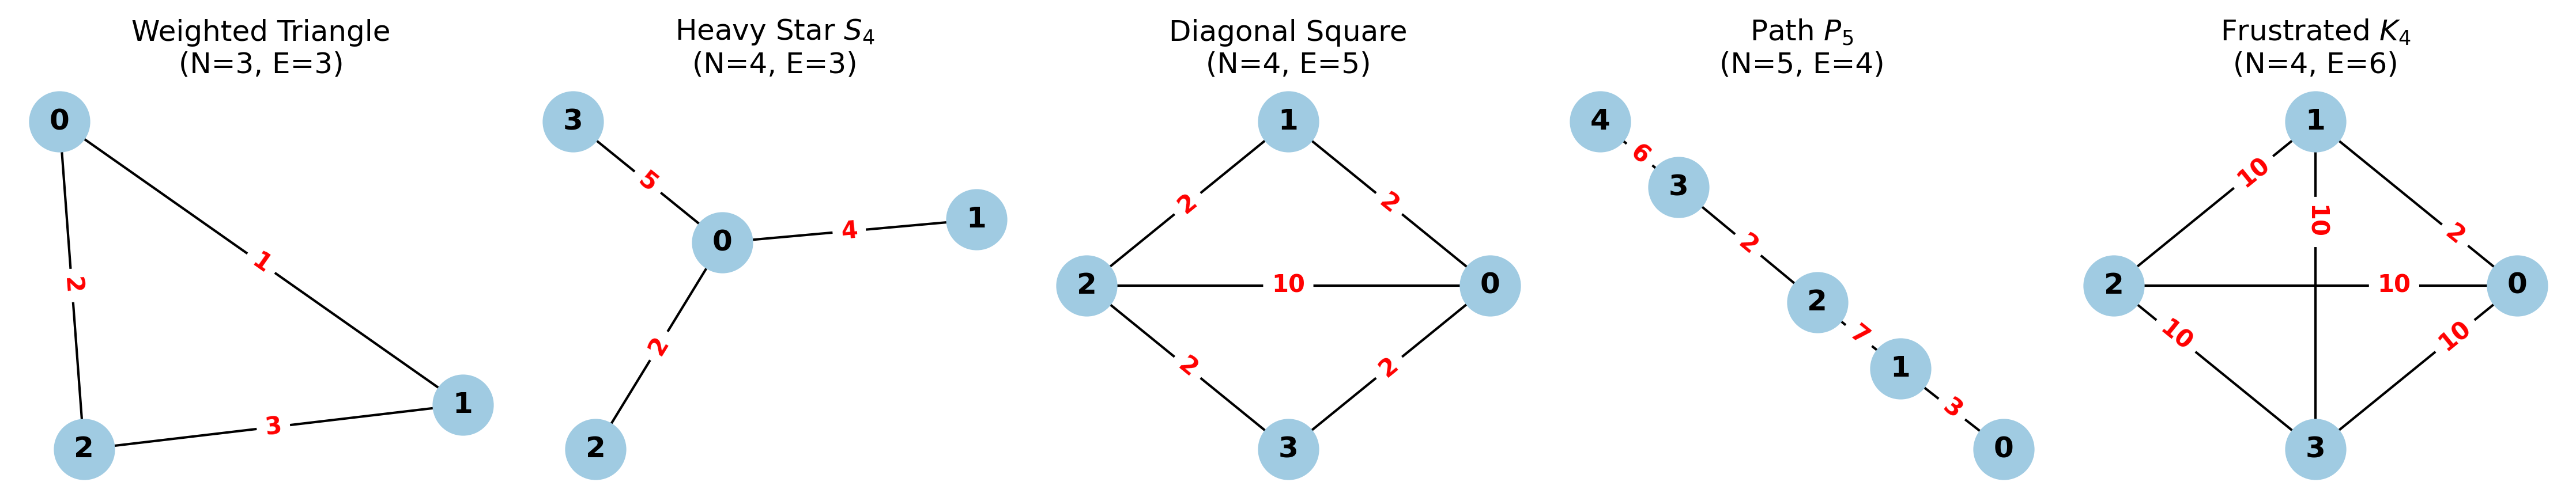
\includegraphics[width=\textwidth]{fig_all_topologies.png}
\caption{Visualization of the five distinct benchmark topologies evaluated in this study. Edge labels denote integer weights representing the varying penalty scales applied to topological collisions.}
\label{fig:topologies}
\end{figure*}

As visualized in Fig.~\ref{fig:topologies}, these five graphs collectively exercise every critical pathological condition: cyclic interference, centralized bottleneck routing, dominant-weight discrimination, extended spatial diameter, and mathematical frustration.

\subsection{Algorithmic Correctness Validation}
To establish absolute confidence in the oracle's computational fidelity, every quantum measurement output was cross-validated against an exhaustive classical brute-force solver enumerating all $K^N$ configurations. For each topology, we confirmed that the highest-probability bitstring decoded from the quantum measurement exactly corresponds to the globally optimal coloring configuration identified classically. Table~\ref{tab:correctness} summarizes the validation results.

\begin{table}[htbp]
\caption{Correctness Validation: Quantum vs. Classical Brute-Force}
\label{tab:correctness}
\centering
\resizebox{\columnwidth}{!}{%
\begin{tabular}{lccccc}
\toprule
Graph Topology & $K^N$ & Optimal Score & \# Optimal & Grover Iters & Match \\
\midrule
Weighted Triangle & 27 & 6 & 6 & 1 & \checkmark \\
Heavy Star $S_4$ & 81 & 11 & 12 & 1 & \checkmark \\
Diagonal Square & 81 & 18 & 6 & 2 & \checkmark \\
Path $P_5$ & 243 & 18 & 16 & 1 & \checkmark \\
Frustrated $K_4$ & 81 & 22 & 6 & 2 & \checkmark \\
\bottomrule
\end{tabular}%
}
\end{table}

Across all five topologies and all three oracle variants (Min Width, Min Depth, Balanced), the quantum algorithm consistently identified the exact global maximum with dominant measurement probability. The Frustrated $K_4$ row is the qualitative point here: Belletti-style Boolean oracles phase-mark only proper colourings and therefore return zero amplitude on this graph by construction, since no proper $3$-coloring exists. The MSB-Overflow oracle instead encodes the optimisation problem (``maximise the weight of properly coloured edges'') rather than the decision problem (``is the colouring proper everywhere?'')---the two oracles solve different problems, and the comparison only makes sense once that framing difference is acknowledged. On non-frustrated graphs the two coincide on which states they mark; on frustrated graphs the MSB-Overflow oracle is the only one that returns a usable answer.

Fig.~\ref{fig:measurement} visualizes the Grover measurement probability distribution for the Frustrated $K_4$ topology, confirming that target optimal configurations are amplified to dominant probabilities well above the uniform baseline.

\Figure[t!](topskip=0pt, botskip=0pt, midskip=0pt)[width=\columnwidth]{fig_measurement.png}
{Grover measurement outcome distribution for the Frustrated $K_4$ graph ($K\!=\!3$, 2 iterations) with edge weights $\{(0,1,10),(0,2,10),(0,3,10),(1,2,10),(1,3,10),(2,3,2)\}$ as used throughout the benchmark suite (Section~\ref{sec:benchmarks}). The total possible weight is $W_{\max}=52$, giving the accumulator width $S = \lceil\log_2(53)\rceil + 1 = 7$ reported in Table~\ref{tab:tgate}. The achievable optimum is $50$ (the only frustrated edge is the lightest, weight $2$), which the oracle identifies through MSB overflow. The x-axis is the raw quantum bitstring measurement, which maps directly to the corresponding graph coloring; green bars indicate the optimum-scoring states, amplified to dominant probability. The dashed red line marks the uniform baseline $1/K^N = 1/81$.\label{fig:measurement}}

\subsection{Transpiled Circuit Metrics}
We extracted the exact spatial and temporal execution metrics for a single Grover iterator ($G = -\mathcal{A}_{\text{init}} S_0 \mathcal{A}_{\text{init}}^{-1} S_f$). The reported depth is the depth of the \emph{full} iterator $G$ after transpilation, i.e.\ it includes the compute pass, the phase-kickback CNOT, the per-edge uncomputation of all collision-check ancillas and Carry-Ripple adders (Algorithm~\ref{alg:oracle}, lines~14--18), and the diffusion operator $\mathcal{A}_{\text{init}} S_0 \mathcal{A}_{\text{init}}^{-1}$; we do not separate compute-only and uncompute halves. Per-iteration cost can be approximately halved to obtain the forward arithmetic path. Table~\ref{tab:results_n} details the empirical qubit width and transpiled circuit depth for all three oracle variants across all five topologies.

\begin{table}[htbp]
\caption{Empirical Space-Time Compilation (Single Grover Iteration)}
\label{tab:results_n}
\centering
\resizebox{\columnwidth}{!}{%
\begin{tabular}{lcccccccc}
\toprule
\multirow{2}{*}{Graph} & \multirow{2}{*}{$(N, E)$} & \multicolumn{2}{c}{Min Width} & \multicolumn{2}{c}{Min Depth} & \multicolumn{2}{c}{Balanced ($C^*$)} \\
\cmidrule(lr){3-4} \cmidrule(lr){5-6} \cmidrule(lr){7-8}
 & & Qubits & Depth & Qubits & Depth & Qubits & Depth \\
\midrule
Triangle & (3, 3) & 12 & 718 & 14 & 640 & 14 & 711 \\
Star $S_4$ & (4, 3) & 15 & 874 & 17 & 794 & 17 & 815 \\
Diag Square & (4, 5) & 16 & 2020 & 20 & 1849 & 19 & 1995 \\
Path $P_5$ & (5, 4) & 18 & 2956 & 21 & 2832 & 20 & 2950 \\
Frustrated $K_4$ & (4, 6) & 17 & 4274 & 22 & 4157 & 20 & 4292 \\
\bottomrule
\end{tabular}%
}
\end{table}

The three variants expose a width--depth trade-off continuum:

1) \emph{Min Width} achieves the tightest qubit footprint ($Q_{MW} = N \cdot q + S + 2$) by recycling a single edge-evaluation ancilla, but at the cost of the deepest critical path. It is the appropriate choice for the most qubit-constrained backends, provided the coherence budget can absorb the extra depth.

2) \emph{Min Depth} allocates independent ancillae per edge ($Q_{MD} = N \cdot q + S + |E| + 1$), enabling the collision-check stage to evaluate every edge in a single layer rather than serially. Empirically this yields a modest depth reduction in the present ripple-carry adder design---ranging from $\sim 11\%$ on the small Triangle graph down to $\sim 3\%$ on Frustrated $K_4$---because the score accumulator is still mutated by serial $\textsc{Add}(w_e)$ operations on a shared register. The gain becomes more significant on graphs where the collision-check stage dominates the per-edge cost, and grows further when the addition stage itself is parallelized (e.g.\ via carry-save or partial-sum-tree adders), which we leave to future work.

Even at the current modest depth reduction, the absolute coherence comparison is illustrative. IBM's Heron processors report median $T_1 \approx 180~\mu\mathrm{s}$ and $T_2 \approx 200~\mu\mathrm{s}$ with a native CX gate time of $\sim 60~\mathrm{ns}$ \cite{ibmheron}. The Frustrated $K_4$ Min Width depth of $4274$ CX-equivalent layers maps to $\sim 256~\mu\mathrm{s}$---already exceeding $T_1$ for a single iteration. The Min Depth circuit at depth $4157$ ($\sim 249~\mu\mathrm{s}$) still does not fit within a single-$T_1$ window, confirming that depth-parallel arithmetic (beyond the per-edge ancilla parallelism captured here) will be required before multi-iteration Grover amplification is feasible on this generation of hardware. As a sanity check on the predictive fit of Eq.~\eqref{eq:depth_fit}, plugging Frustrated $K_4$ ($|E|=6$, $S=7$) into $D_{MW} \approx \kappa \cdot |E| \cdot S^2$ with the lower-$N$ value $\kappa \approx 14.5$ yields a predicted depth of $\sim 4{,}260$, within $0.3\%$ of the measured $4{,}274$.

3) \emph{Balanced} deploys $C^{*} = \lceil(1 + \sqrt{8E-7})/2\rceil$ recycling ancillae, interpolating between the two extremes. For Frustrated $K_4$ with $C^* = 4$, it lands within $1\%$ of the Min Width depth while costing only $3$ additional qubits, so its primary value is operational---it removes the need to hand-tune $C$ per graph---rather than a depth win in this regime.

\subsection{Empirical Scaling Beyond the Paper Benchmark}
\label{sec:scaling_measured}

To extend Table~\ref{tab:results_n} past the $N{=}3$--$5$ regime that the named topologies cover, we generated random connected graphs with $N \in \{6,\,8,\,10,\,12\}$ vertices, $|E| \approx 2.4\,N$ edges, $K = 3$ colors, and integer edge weights drawn uniformly from $[1,\,10]$. For each $N$ we used two independent random seeds and transpiled every oracle variant through the same Qiskit pipeline used for Table~\ref{tab:results_n}. Brute-force ground truth is enumerated classically ($K^N \le 5.3 \times 10^5$). The generator and transpilation harness are released as \texttt{extend\_table\_scaling.py}; Table~\ref{tab:scaling_measured} reports the per-seed measurements.

\begin{table}[htbp]
\caption{Empirical Scaling for Random Moderate-Density Graphs ($K=3$, weights in $[1,10]$, 1 Grover iteration)}
\label{tab:scaling_measured}
\centering
\resizebox{\columnwidth}{!}{%
\begin{tabular}{ccccccccc}
\toprule
\multirow{2}{*}{$N$} & \multirow{2}{*}{$|E|$} & \multirow{2}{*}{seed} & \multirow{2}{*}{$S$} & \multicolumn{2}{c}{Min Width} & \multicolumn{2}{c}{Min Depth} & Balanced \\
\cmidrule(lr){5-6} \cmidrule(lr){7-8}
 & & & & $Q$ & Depth & $Q$ & Depth & $Q$ / Depth \\
\midrule
6  & 15 & 11 & 7 & 21 & 11{,}554 & 35 & 11{,}086 & 26 / 11{,}419 \\
6  & 15 & 23 & 8 & 22 & 18{,}437 & 36 & 17{,}927 & 27 / 18{,}248 \\
8  & 20 & 11 & 8 & 26 & 23{,}899 & 45 & 23{,}291 & 32 / 23{,}665 \\
8  & 20 & 23 & 8 & 26 & 24{,}916 & 45 & 24{,}311 & 32 / 24{,}732 \\
10 & 24 & 11 & 8 & 30 & 27{,}552 & 53 & 27{,}106 & 37 / 27{,}427 \\
10 & 24 & 23 & 9 & 31 & 38{,}274 & 54 & 37{,}913 & 38 / 38{,}345 \\
12 & 29 & 11 & 9 & 35 & 48{,}155 & 63 & 47{,}521 & 42 / 47{,}646 \\
12 & 29 & 23 & 9 & 35 & 48{,}320 & 63 & 47{,}712 & 42 / 48{,}223 \\
\bottomrule
\end{tabular}%
}
\end{table}

The measurements confirm the formulas of Section~\ref{sec:formulation} across the wider range: every $Q$ value matches $N \cdot q + S + 2$, $N \cdot q + S + |E| + 1$, and $N \cdot q + S + C^* + 1$ respectively, with $q = 2$ for $K = 3$. The depth column also confirms the trend identified at $N=3$--$5$: Min Depth offers only a $1$--$4\%$ improvement over Min Width across the eight graphs (e.g.\ $N{=}12$: $48{,}155 \to 47{,}521$, a $1.3\%$ reduction), because the ripple-carry additions still serialise on the shared accumulator regardless of how many edge ancillae are allocated. Realising the larger gains assumed by Table~\ref{tab:scalability} for the $N=20, 50, 100$ projections requires the depth-parallel adder variants discussed in Section~\ref{sec:practical_limits}.

For practical estimation, the eight measurements admit a tight empirical fit
\begin{equation}
D_{MW} \approx \kappa \cdot |E| \cdot S^2, \qquad \kappa \in [15.7,\, 20.6],
\label{eq:depth_fit}
\end{equation}
with the constant rising from $\kappa \approx 16$ at $N=6$ to $\kappa \approx 20.5$ at $N=12$ as the diffusion operator and the Custom State Preparation contribute a slowly-growing $N$-dependent overhead on top of the per-edge arithmetic. The same fit reproduces $D_{MD}$ within $5\%$ across all eight rows, consistent with the practical observation above that $D_{MD}$ and $D_{MW}$ share the $|E| \cdot S^2$ scaling under the current ripple-carry implementation. Equation~\eqref{eq:depth_fit} is the practical formula to use when sizing the oracle for a given hardware coherence budget; the asymptotic forms in Section~\ref{sec:methodology} should be read as the limit toward which a depth-parallel adder implementation would converge.

\subsection{Theoretical Resource Estimations}
Beyond the compiler transpilation outputs, establishing generalized theoretical scaling parameters—specifically regarding total gate counts, Toffoli operations, and $T$-gate metrics—is critical for evaluating future fault-tolerant integration trajectories.

\paragraph{Asymptotic Total Gate Count}
The total gate count of the MSB-Overflow Oracle is determined by three components: state preparation, edge collision checking, and weight accumulation. State preparation costs $\mathcal{O}(\log_2 K)$ gates per node, totalling $\mathcal{O}(N \log_2 K)$. Each of the $|E|$ edges uses a $q$-bit comparator of $\mathcal{O}(\log_2 K)$ gates followed by a ripple-carry adder linear in the accumulator width $S = \mathcal{O}(\log_2 W_{\max})$. The phase-kickback layer contributes a single CNOT. The total per-iteration gate count is therefore:
\begin{equation}
\mathcal{O}\big(N \log_2 K + |E| \cdot (\log_2 K + \log_2 W_{\max})\big)
\label{eq:asymptotic_gate}
\end{equation}

\paragraph{T-gate Estimations \& Baseline Comparison}
The standard ripple-carry quantum adders utilized in our architecture demand roughly $4S$ Toffoli (CCX) operations per discrete edge addition, where $S$ is the accumulator bit-width. Because each standard Toffoli decompiles into $7$ distinct $T$-gates, the theoretical $T$-count bound scales as $\mathcal{O}(28S \cdot |E|)$ for the adder arithmetic alone. Additionally, the edge comparison subcircuit for each edge requires $q = \lceil \log_2 K \rceil$ Toffoli gates. Table~\ref{tab:tgate} summarizes the resource estimations across all benchmark topologies.

Compared to the Boolean formulation of Belletti \textit{et al.}~\cite{belletti2025}, our architecture removes one asymptotic term and adds another. Belletti's unweighted oracle places invalid-colour checkers on every node, yielding a Toffoli density of $\mathcal{O}((|V| + |E|) \log_2 K)$. Pruning phantom states at initialisation and replacing the multi-controlled phase validation with a single CNOT eliminates the $\mathcal{O}(|V| \log_2 K)$ invalid-colour term; it is replaced by the $\mathcal{O}(\log_2 W_{\max})$ adder overhead intrinsic to the MWCSP.

\begin{table}[htbp]
\caption{Theoretical Toffoli and $T$-Gate Estimations (Per Grover Iteration)}
\label{tab:tgate}
\centering
\resizebox{\columnwidth}{!}{%
\begin{tabular}{lccccc}
\toprule
Graph & Acc. Width ($S$) & Toffoli (Adder) & Toffoli (Compare) & $T$-count (Total) \\
\midrule
Weighted Triangle & 4 & 48 & 6 & 378 \\
Heavy Star $S_4$ & 5 & 60 & 6 & 462 \\
Diagonal Square & 6 & 120 & 10 & 910 \\
Path $P_5$ & 6 & 96 & 8 & 728 \\
Frustrated $K_4$ & 7 & 168 & 12 & 1260 \\
\bottomrule
\end{tabular}%
}
\end{table}

\subsection{MSB-Overflow Comparator Depth Reduction}
The most significant architectural advantage of the proposed MSB-Overflow mechanism is the reduction in the \emph{comparator subcircuit} depth. Traditional exact-match comparators require deploying a dense $S$-qubit MCX gate that decompiles into $\mathcal{O}(S^2)$ sequential operations under nearest-neighbor connectivity constraints. Our Overflow-Flag approach replaces this entirely with a single CNOT gate applied to the MSB flag qubit. Concretely, across the five benchmark topologies (with $S$ ranging from $4$ to $7$), the comparator block contributes $\mathcal{O}(S^2) \in [16, 49]$ sequential operations under the traditional formulation, compared to a single CNOT under our design---yielding a comparator-block depth reduction of roughly $16\times$ to $49\times$ (mean $\approx 30\times$). This is the depth reduction of the comparator stage in isolation; the full-circuit depth reduction is necessarily smaller because the ripple-carry adder stages remain the dominant per-iteration cost.

\subsection{Quantitative Comparison with the Belletti Baseline}
\label{sec:belletti_quant}

Section~\ref{sec:qarith_related} and the asymptotic discussion above frame Belletti's design only in big-$\mathcal{O}$ terms. For a direct, like-for-like resource comparison we reimplemented a Belletti-style Boolean oracle in Qiskit---generic Hadamard initialisation, per-node invalid-colour checker, per-edge collision detector, and a global MCX phase trigger over all $|V|+|E|$ flag ancillas, with full uncomputation as in our own oracle---and transpiled it through the identical pipeline used for Table~\ref{tab:results_n} (basis $\{cx, id, rz, sx, x\}$, \texttt{optimization\_level=3}). Code is released in the supplementary repository as \texttt{belletti\_baseline.py}.

Belletti's oracle is strictly unweighted (it phase-marks a colouring iff every edge satisfies $C(u) \ne C(v)$ and no node holds a phantom colour) and therefore cannot represent the MWCSP target $T$ at all; on Frustrated $K_4$ it returns zero amplitude by construction because no proper $3$-coloring exists. The comparison in Table~\ref{tab:belletti_compare} is therefore a resource-only comparison per Grover iteration, not a quality comparison. The reading is straightforward: Belletti uses fewer ancillas and shorter circuits in the unweighted regime where it works, and our oracle pays a deterministic overhead---one accumulator register of width $S = \lceil \log_2(W_{\max}+1) \rceil + 1$ and a per-edge ripple-carry adder---to gain weight handling and frustration tolerance.

\begin{table}[htbp]
\caption{Belletti unweighted baseline vs.\ MSB-Overflow (Min Width), per Grover iteration. Both circuits transpiled through Qiskit \texttt{optimization\_level=3} on the same basis gate set. Belletti's oracle phase-marks only proper colourings and is incapable of representing weights or returning non-zero amplitude on Frustrated $K_4$; the columns therefore report resource consumption only.}
\label{tab:belletti_compare}
\centering
\resizebox{\columnwidth}{!}{%
\begin{tabular}{lccccc}
\toprule
\multirow{2}{*}{Graph} & \multirow{2}{*}{$(N, E)$} & \multicolumn{2}{c}{Belletti (unweighted)} & \multicolumn{2}{c}{MSB-Overflow MW (weighted)} \\
\cmidrule(lr){3-4} \cmidrule(lr){5-6}
 & & Qubits & Depth & Qubits & Depth \\
\midrule
Triangle         & (3, 3) & 13 & 272 & 12 & 718  \\
Star $S_4$       & (4, 3) & 16 & 337 & 15 & 874  \\
Diag Square      & (4, 5) & 18 & 442 & 16 & 2020 \\
Path $P_5$       & (5, 4) & 20 & 443 & 18 & 2956 \\
Frustrated $K_4$ & (4, 6) & 19 & 468 & 17 & 4274 \\
\bottomrule
\end{tabular}%
}
\end{table}

The Belletti qubit count matches the closed form $Nq + |V| + |E| + 1$ across all five rows; ours matches $Q_{MW} = Nq + S + 2$ (Section~\ref{sec:methodology}). On the qubit axis we save $1$--$2$ qubits because we exchange $|V|+|E|$ per-node/per-edge flag ancillas for one $S$-wide accumulator. On the depth axis we pay between $2.6\times$ (Triangle) and $9.1\times$ (Frustrated $K_4$): the overhead is dominated by the per-edge ripple-carry $\textsc{Add}(w_e)$ and its uncomputation, which Belletti does not execute. This depth is what enables the oracle to do something Belletti cannot, namely return a maximum-weight partial colouring on a frustrated graph (Section~\ref{sec:benchmarks}, Table~\ref{tab:correctness}).


\subsection{Empirical Behaviour under Depolarising Noise}
\label{sec:noise_sweep}

The correctness validation in Section~\ref{sec:benchmarks} runs on a noiseless Aer simulator. To put the depth numbers from Table~\ref{tab:results_n} into hardware context, we re-ran the Min Width oracle through a depolarising noise model parameterised against the publicly reported median characteristics of IBM Heron-class processors: $T_1 \approx 180~\mu\mathrm{s}$, $T_2 \approx 200~\mu\mathrm{s}$, CX gate time $\sim 60~\mathrm{ns}$, two-qubit Pauli error $5\times 10^{-3}$, and single-qubit error $\sim 2 \times 10^{-4}$. We sweep an overall error-rate scale of $\{0\text{ (ideal)},\,0.25,\,1.0,\,4.0\}$ relative to those baseline numbers; $4.0$ corresponds to roughly the worst-case Eagle/Heron pre-calibration regime, and $0.25$ approximates an aggressive future-generation device. All circuits use a single Grover iteration with the optimal classical Target. Sampled probabilities are computed over $4{,}096$ shots; the script is included as \texttt{noisy\_simulation.py} for reproducibility.

\begin{table}[htbp]
\caption{Min Width Oracle: $P(\text{measure optimal coloring})$ vs.\ Depolarising Noise Scale}
\label{tab:noisy}
\centering
\resizebox{\columnwidth}{!}{%
\begin{tabular}{lccccc}
\toprule
\multirow{2}{*}{Graph} & \multirow{2}{*}{Depth} & \multicolumn{4}{c}{$P_{\text{opt}}$ at noise scale} \\
\cmidrule(lr){3-6}
 & & $0$ (ideal) & $0.25\times$ & $1.0\times$ & $4.0\times$ \\
\midrule
Triangle    & 718  & 0.991 & 0.760 & 0.435 & 0.369 \\
Star $S_4$  & 874  & 0.977 & 0.696 & 0.416 & 0.420 \\
Diag Square & 2020 & 0.527 & 0.269 & 0.172 & 0.188 \\
\bottomrule
\end{tabular}%
}
\end{table}

The behaviour clearly stratifies by depth. For Triangle ($D{=}718$) and Star $S_4$ ($D{=}874$), the ideal probability stays above $97\%$ and the Heron-baseline ($1.0\times$) probability stays at roughly $0.42$---comfortably above the uniform baselines $1/K^N$ of $0.037$ and $0.012$ respectively, so the oracle still amplifies the optimal subspace meaningfully on present hardware. For Diagonal Square ($D{=}2020$), the ideal probability is already $0.527$ (a single Grover iteration is sub-optimal for this graph, which classically supports $|\mathcal{S}^*|{=}6$ optima and would benefit from $R{=}2$), and at Heron baseline it collapses to $0.172$, less than half the ideal value. At the $4.0\times$ scale the probabilities flatten in the range $0.18$--$0.42$, which is the residual mixing floor where the channel has decohered the accumulator into a near-maximally-mixed state and the measurement projects onto the unaltered superposition of valid colorings.

Two implications follow. First, the depth-vs.\ width trade-off discussed in Section~\ref{sec:formulation} is not just a coherence-budget abstraction: a Min Width circuit at depth $\sim 2{,}000$ already approaches the practical noise floor on Heron-class hardware, so the Min Depth and Balanced variants---despite costing more qubits---are the only candidates that may close the gap on a physical device before fault-tolerant error correction is available. Second, the deeper benchmark topologies (Path $P_5$ and Frustrated $K_4$, with depths $2{,}956$ and $4{,}274$) sit well past the regime where this noise model preserves a useful signal; we omit them from Table~\ref{tab:noisy} because their Heron-baseline probabilities sit indistinguishably at the uniform floor in our shot-budget. Reaching those topologies on physical hardware therefore requires logical encoding rather than raw NISQ execution---directly motivating the fault-tolerant resource estimates in Section~V.

\subsection{Comparison with QAOA: Analog Approximations vs. Digital Exactness}
\label{sec:comparison}
When benchmarking our exact formulation against standard heuristic equivalents like QAOA, three critical structural advantages emerge:

\paragraph{Exactness Guarantee}
QAOA formally possesses no mathematical guarantee of converging onto the global maximum. Its solutions are bounded by an approximation ratio dependent on the layered circuit depth $p$, with the optimum amplitude in general inaccessible from any fixed $(p, \gamma, \beta)$ schedule. In contrast, our Overflow-Flag Grover Oracle amplifies the optimal subspace to its closed-form Grover saturation $\sin^2((2R{+}1)\theta)$ with $\theta = \arcsin\sqrt{|\mathcal{S}^*|/M}$ at the optimal iteration count $R = \lfloor \frac{\pi}{4}\sqrt{M / |\mathcal{S}^*|} \rfloor$, where $|\mathcal{S}^*|$ is the number of optimal solutions. This saturation is independent of any classical optimiser and yields the empirically observed $\ge 96\%$ per-shot success rates reported in Table~\ref{tab:empirical_scaling}; the small residual on non-optimal configurations is the standard Grover amplitude leftover at finite $R$, not a convergence failure.

\paragraph{Classical Loop Elimination}
QAOA's performance is bottlenecked by classical optimization loops (COBYLA, Nelder-Mead) configuring continuous Hamiltonian angles ($\boldsymbol{\gamma}, \boldsymbol{\beta}$). Research establishes that optimizing these gradients against densely connected topologies frequently traps the solver in barren plateaus \cite{mcclean2018barren}, where the gradient variance vanishes as $\mathcal{O}(2^{-N})$. Our architecture requires precisely zero classical tuning loops; the classical pre-computation is bounded by $\mathcal{O}(1)$.

\paragraph{Mathematical Encoding Divergence \& The Quadratic Constraint Wall}
While our proposed MSB-Overflow architecture utilizes explicit digital arithmetic to natively accumulate edge weights, QAOA relies on mapping the MWCSP into a Quadratic Unconstrained Binary Optimization (QUBO) model or Ising Hamiltonian. This architectural reliance introduces a severe scaling bottleneck: QUBO formulations inherently restrict variable interactions to a maximum of 2-body (quadratic) terms to remain physically compatible with 2-qubit native hardware operations (e.g., $ZZ$ interactions). 

If one were to attempt mapping the MWCSP using a space-efficient binary encoding ($\lceil \log_2 K \rceil$ qubits per node), evaluating whether two nodes share the same color would require calculating algebraic equivalents of $XNOR$ logic across multiple qubits. Expanding these boolean algebraic equations mathematically produces higher-order terms (e.g., 4-body interactions for $K=4$, or 6-body for $K=8$). Because native hardware cannot execute 4-body Hamiltonians without deploying complex, resource-heavy quadratization gadgets and massive auxiliary penalties, QAOA architectures are forced to abandon binary encoding entirely.

Consequently, QAOA typically adopts \textit{one-hot encoding} ($K$ qubits per node), ensuring the color-collision penalty remains structurally quadratic: $w_{ij} \sum_k x_{i,k} x_{j,k}$. This encoding choice significantly expands the Hilbert space to $2^{K \cdot |V|}$. For a $P_5$ graph with $K=3$ colors, the space expands to $32{,}768$ states, of which only $243$ ($<0.75\%$) are valid. To enforce the one-hot rule, a large penalty term ($A \sum (1 - \sum x)^2$) must be applied. The standard QAOA transverse-field mixer ($H_B = \sum X_i$) is not aware of these constraints, and can drive the system away from the valid subspace.

In contrast, our Grover-based digital architecture effectively bypasses the QUBO restriction. By synthesizing explicit quantum boolean logic (cascading Toffoli gates), our architecture handles higher-order comparisons directly in the digital domain. This allows the MSB-Overflow oracle to utilize a dense, space-efficient binary encoding ($|V|\lceil \log_2 K \rceil$) while eliminating the need for penalty Hamiltonians, yielding a $100\%$ valid search space by construction.

\paragraph{Methodological \& Architectural Comparison}
The two approaches occupy different asymptotic regimes. QAOA uses fewer physical qubits because its variable mapping is $\mathcal{O}(|V|)$, but it has no mechanism to guarantee an approximation ratio of $\alpha = 1$: at $p{=}1$ the depth is small but the bound on $\alpha$ is loose, and on frustrated graphs the bound degrades further. Increasing $p$ to tighten $\alpha$ runs into the barren-plateau problem for graphs with $N > 10$~\cite{mcclean2018barren}, where the classical optimiser stalls. Our Grover oracle takes the opposite trade: spatial complexity $\mathcal{O}(|E| + |V|\log_2 K)$ in exchange for immunity to barren plateaus and a fixed-amplification schedule that places $\ge 96\%$ of the per-shot probability on the global optimum at the optimal $R$ (Table~\ref{tab:empirical_scaling}), independent of any classical optimiser.

Crucially, the significant impact of this penalty trap is empirically observable. To ensure a rigorous baseline comparison, we evaluated QAOA against our paper's core topologies utilizing exact statevector simulations with a deep ansatz ($p = 7$) and intensive multi-seed L-BFGS-B optimization. The exact configuration that produced the numbers in Table~\ref{tab:empirical_scaling} is as follows: one-hot encoding with $K = 3$ colors per vertex, penalty Hamiltonian coefficient $\lambda = 15.0$ enforcing the one-hot constraint, $5$ independent restarts per topology with QAOA angles initialized uniformly at random in $[-\pi, \pi]^{2p}$, master NumPy seed $99$ for reproducibility, and L-BFGS-B from \texttt{scipy.optimize.minimize} with $\mathtt{maxiter}=300$ at the SciPy default convergence tolerances ($\mathtt{gtol}=10^{-5}$, $\mathtt{ftol}\approx 2.22 \times 10^{-9}$). We keep the best of the $5$ restarts (lowest expected cost) per topology and report its single-shot statistics in the table. The exact script, including the Ising encoder, the cost function, and the optimization driver, is released as \texttt{qaoa\_depth\_sweep.py} in the supplementary repository.
This noise-free environment isolates the theoretical capacity of the algorithm by entirely removing hardware-induced finite-sampling variance. We report a single concrete metric in Table~\ref{tab:empirical_scaling}: the number of measurement outcomes that decode to a globally optimal coloring out of $2048$ independent computational-basis measurements drawn from each algorithm's final, noise-free statevector. Concretely, the circuit---the QAOA ansatz at $p=7$ for the QAOA column, or the complete Grover schedule with the empirically-optimal iteration count $R$ for the MSB-Overflow column---is executed once on Qiskit's Aer simulator, and the resulting amplitude distribution over the computational basis is sampled $2048$ times. Each sample is a bitstring decoded into a node-coloring tuple $(C(v_1), \dots, C(v_N))$, whose score $\sum_{(u,v) \in E} w_{(u,v)} \cdot \mathbb{1}[C(u){\ne}C(v)]$ is then compared against the brute-force classical optimum; a \emph{hit} is any sample whose decoded score equals the optimum. The 2048-shot budget is identical for both architectures, so the comparison is directly operational---reading off the table tells you, per topology, how many of $2048$ measurements you can expect to recover the optimum from each approach. Note that we deliberately do not report the conventional QAOA approximation ratio $\alpha = \langle C \rangle / C_{\mathrm{opt}}$ because the penalty Hamiltonian biases $\langle C \rangle$ toward infeasible states with negative cost contributions, which is an artefact of the QUBO encoding rather than a measure of algorithmic quality. Even under mathematically optimal noise-free conditions, the heuristic approach exhibits a significant degradation in state validity on constrained graphs. For the $P_5$ topology, over 90\% of the probability amplitude remains trapped in physically invalid (non-one-hot) states, restricting the QAOA single-shot success rate to roughly $4.6\%$, which translates to only $95$ optimal outcomes per $2048$ shots versus $1{,}974$ for the MSB-Overflow run on the same shot budget.

By contrast, our MSB-Overflow oracle guarantees $100\%$ state validity \textit{by construction} via its custom state preparation, bypassing the probabilistic penalty issue. While QAOA requires fewer operational qubits due to its lack of explicit arithmetic registers, the convergence behaviour above limits its practical applicability on these constrained instances. Our architecture trades a modest spatial overhead ($\approx 2$ to $4$ auxiliary qubits relative to one-hot QAOA) for a fixed-amplitude schedule that recovers the global maximum on $\ge 96\%$ of independent shots at the optimal iteration count $R$ (Table~\ref{tab:empirical_scaling}).

\paragraph{Transpiled Resource Disparity}
To establish a direct, apples-to-apples comparison, both architectures are transpiled to the standard hardware-native basis gate set $\{CX, RZ, SX, X\}$ via Qiskit's preset pass manager (optimization level~3). This represents the exact gate sequence that would be executed on a physical quantum processor. For the QAOA ansatz at $p=7$, transpilation consolidates and optimizes the raw circuit into $713$--$1{,}130$ hardware-native gates across our benchmark topologies. Although this count appears modest, the critical limitation is not gate count but the \textit{cost of reaching a given success probability}: even under mathematically ideal statevector simulation, QAOA recovers only $67$--$454$ optimal outcomes out of $2048$ shots across our benchmark topologies, while producing invalid (non-one-hot) states at rates exceeding $90\%$ for larger topologies (Table~\ref{tab:empirical_scaling}).

Conversely, our MSB-Overflow oracle, transpiled through the identical pass manager, decomposes its Toffoli-based arithmetic into an equivalent hardware-native gate sequence. The total transpiled gate count for our architecture encapsulates the \textit{entire} deterministic search algorithm, including all optimal Grover iterations $R$ (chosen empirically per topology to maximise per-shot success). While the MSB-Overflow architecture requires a moderately higher transpiled gate count due to its explicit arithmetic registers, this overhead purchases a near-deterministic outcome: across all five topologies, $1{,}967$--$2{,}028$ of $2048$ shots ($\ge 96\%$) decode to a globally optimal coloring, with the small shortfall from the $2048$-shot ceiling reflecting the residual amplitude that Grover amplification leaves on non-optimal configurations at any finite $R$.

\paragraph{Positioning Against Recent Hybrid Approaches}
Recent work by Liu \textit{et al.}~\cite{liu2025hybrid} proposes a hierarchical hybrid QAOA framework for unweighted graph coloring that uses binary encoding ($\lceil \log_2 K \rceil$ qubits per node) to reduce qubit requirements. Their approach partitions large graphs via a balanced community detection algorithm, applies QAOA independently to small subgraphs ($V_{sub} \le \lfloor Q / \lceil \log_2 K \rceil \rfloor$), and resolves inter-partition conflicts through classical greedy post-processing. The binary encoding reduces qubit count compared to one-hot QAOA, but their soft-constraint color-equality term, stated as $H_{\text{edge}}^{(u,v)} = \sum_{i=0}^{m-1} (I - Z_{u,i} \otimes Z_{v,i})$ in their Eq.~(10), is a sum-of-per-bit Hamming weight rather than an exact color comparator. Two distinct colors whose binary encodings differ on a different number of bits therefore contribute different energies even though both correspond to a legitimately satisfied edge. For instance, with $K = 4$ ($m = 2$), the pair $(\texttt{00},\texttt{01})$ and the pair $(\texttt{00},\texttt{11})$ are both valid colorings yet they receive Hamiltonian eigenvalues of $2$ and $4$ respectively, biasing the optimizer toward maximum-Hamming-distance assignments rather than uniform reward across all valid color pairs. The bias is structurally incompatible with the MWCSP because the per-bit term enters the objective scaled by edge weights $w_{ij}$, so heavily weighted edges amplify the encoding artifact rather than the genuine optimization signal. Our MSB-Overflow architecture retains the qubit-count advantage of binary encoding while replacing the soft-constraint approximation with an explicit digital comparator, recovering exact color equality for both weighted and unweighted variants.

\begin{table*}[htbp]
\caption{Empirical Scaling: Exact Transpiled Gate Counts and Sampled Success at 2048 Shots for QAOA ($p=7$) vs.\ MSB-Overflow. \textbf{Hits / 2048} ($\uparrow$, higher is better) is the empirical number of measurement outcomes that decode to a globally optimal coloring out of $2048$ independent shots drawn from the noise-free statevector, and \textbf{Success Rate} is the same quantity expressed as a percentage. For QAOA this counts shots of the converged $p=7$ ansatz; for MSB-Overflow this counts shots of a single complete Grover run at the empirically-optimal iteration count $R$. The MSB-Overflow figures stay below the theoretical ceiling of $2048$ because Grover amplification leaves residual amplitude on non-optimal configurations even at the optimal $R$.}
\label{tab:empirical_scaling}
\centering
\renewcommand{\arraystretch}{1.3}
\resizebox{\textwidth}{!}{%
\begin{tabular}{l cccc cccc}
\toprule
\multirow{2}{*}{\textbf{Topology ($K=3$)}} & \multicolumn{4}{c}{\textbf{QAOA ($p=7$, Exact Statevector)}} & \multicolumn{4}{c}{\textbf{MSB-Overflow (Complete Search)}} \\
\cmidrule(lr){2-5} \cmidrule(lr){6-9}
& \textbf{Qubits} & \textbf{Trans. Gates} & \textbf{Hits / 2048} $\uparrow$ & \textbf{Success Rate} $\uparrow$
& \textbf{Qubits} & \textbf{Trans. Gates} & \textbf{Hits / 2048} $\uparrow$ & \textbf{Success Rate} $\uparrow$ \\
\midrule
Weighted Triangle & 9  & 713    & 312 & $15.23\%$ & 12 & \textbf{3{,}456}  & \textbf{2{,}028} & $\mathbf{99.02\%}$ \\
Heavy Star $S_4$  & 12 & 890    & 454 & $22.17\%$ & 15 & \textbf{3{,}696}  & \textbf{1{,}996} & $\mathbf{97.46\%}$ \\
Diagonal Square   & 12 & 1{,}016  & 67  & $3.27\%$  & 16 & \textbf{12{,}320} & \textbf{1{,}967} & $\mathbf{96.05\%}$ \\
Frustrated $K_4$  & 12 & 1{,}079  & 68  & $3.32\%$  & 17 & \textbf{17{,}472} & \textbf{1{,}971} & $\mathbf{96.24\%}$ \\
Path $P_5$        & 15 & 1{,}130  & 95  & $4.64\%$  & 18 & \textbf{5{,}632}  & \textbf{1{,}974} & $\mathbf{96.39\%}$ \\
\bottomrule
\end{tabular}%
}
\end{table*}

\subsection{Practical Limits and Total-Runtime Considerations}
\label{sec:practical_limits}

The per-iteration depth reduction reported above must be interpreted in the context of Grover's overall runtime. For an unstructured search over $M = K^N$ configurations with $|\mathcal{S}^*|$ optimal targets, the optimal iteration count is
\begin{equation}
R = \left\lfloor \frac{\pi}{4} \sqrt{M / |\mathcal{S}^*|} \right\rfloor,
\label{eq:grover_iters}
\end{equation}
which remains exponential in $N$ regardless of how aggressively the per-iteration oracle is compressed. The contribution of this paper is therefore best understood as reducing the prefactor in front of the unavoidable $\sqrt{M / |\mathcal{S}^*|}$ scaling, not as eliminating it.

\paragraph{Unknown $|\mathcal{S}^*|$ at deployment time.}
Eq.~\eqref{eq:grover_iters} requires $|\mathcal{S}^*|$ to set $R$, but in a deployed MWCSP instance the number of optimal colourings is generally not known a priori. The standard remedy is the exponential-search wrapper of Brassard~\textit{et al.}~\cite{brassard2002}: run the oracle with $R$ drawn uniformly from $\{0, 1, \dots, \lceil m \rceil - 1\}$, doubling $m$ on each unsuccessful round until a marked configuration is sampled. The wrapper finds a marked state in $\mathcal{O}(\sqrt{M/|\mathcal{S}^*|})$ expected oracle calls without knowing $|\mathcal{S}^*|$ and preserves the $\sqrt{M}$ Grover speedup. In our reported empirical runs we use the empirically-optimal $R$ from Table~\ref{tab:correctness} to isolate the per-iteration oracle cost; a deployed implementation should compose the MSB-Overflow oracle with this exponential-search wrapper, at the cost of a $\log$-factor in the constant.

\paragraph{When does Grover apply?}
For the benchmark topologies in Table~\ref{tab:results_n}, the empirically-optimal $R$ ranges from $1$ to $2$ (Table~\ref{tab:correctness}) and the total CX-equivalent depth of a full run (oracle + diffuser, $R$ iterations) stays below $10^4$ layers---an envelope already achievable on near-term fault-tolerant prototypes. For the speculative regime $N{=}20, |E|{=}30$ in Table~\ref{tab:scalability}, $R \approx \lfloor (\pi/4)\sqrt{3^{20}} \rfloor \approx 1.86 \times 10^5$, and combining with the Min Depth projection yields an aggregate workload near $10^7$ $T$-gates---demanding but plausible for a mature fault-tolerant device. For $N{=}100$, $R \approx 7 \times 10^{23}$, which we acknowledge places the corresponding row of Table~\ref{tab:scalability} firmly outside the regime of any conceivable hardware. We retain the $N \in \{50, 100\}$ projections only to expose the asymptotic shape of the qubit and $T$-gate dependence on graph size, not as feasibility claims.

\paragraph{Determining the Target weight.}
Algorithm~\ref{alg:oracle} accepts the threshold $T$ as a classical input. In a deployed MWCSP instance the true maximum weight is generally unknown a priori, so $T$ must be discovered iteratively. We follow the maximum-finding wrapper of D\"urr and H\o yer~\cite{durr1996minimum}: starting from a candidate threshold $T_0$ obtained from any cheap classical heuristic (e.g.\ greedy coloring), execute the Grover oracle of Algorithm~\ref{alg:oracle} with target $T_0$, measure to obtain a sample configuration $X_0$ with score $s_0 \ge T_0$, set $T_1 \leftarrow s_0 + 1$, and iterate. The outer loop terminates when an oracle invocation returns no measurement satisfying $s \ge T_k$ after the prescribed iteration budget, at which point $T_k - 1$ is the certified maximum. The wrapper preserves the quadratic Grover speedup and adds a $\mathcal{O}(\log_2 W_{\max})$ multiplicative factor in the worst case, since the threshold can rise at most $W_{\max}$ times. The MSB-Overflow construction in this paper is exactly the oracle subroutine consumed by this wrapper; switching between unweighted, weighted, and even minimum-weight variants requires only changing the sign convention of $\mathrm{Offset}$ and the direction of accumulation.

\section{Conclusion \& Future Work}

\subsection{Concluding Remarks}
This paper addresses one structural bottleneck of exact Grover oracles for the MWCSP: the $\mathcal{O}(S^2)$ MCX comparator that exact-match designs place on the critical path of every iteration. Pre-loading the accumulator with the classical offset $\text{Offset} = 2^{S-1} - \text{Target}$ reduces that comparator sub-block to a single CNOT on the MSB, and the Custom State Preparation layer removes the per-node invalid-colour checker subcircuits used by prior designs.

We are careful to distinguish the comparator-stage saving from the full-circuit cost. Two MCX-heavy blocks remain on the per-iteration critical path: (i) the per-edge ripple-carry $\textsc{Add}(w_e)$, which is intrinsic to the weighted formulation and now dominates the transpiled depth, and (ii) the standard Grover diffusion operator $\mathcal{A}_\mathrm{init} S_0 \mathcal{A}_\mathrm{init}^{-1}$, whose $S_0$ block still contains a multi-controlled phase on the $N q$ coloring qubits. The empirical fit $D_{MW} \approx \kappa \cdot |E| \cdot S^2$ extracted in Section~\ref{sec:scaling_measured} reflects these two terms, not the comparator. Against the Belletti Boolean baseline, the resulting net trade is $1$--$2$ qubits saved at the cost of $2.6\times$--$9.1\times$ depth, with the depth penalty coming from the adder block, not the new comparator. We therefore frame the contribution as a depth-prefactor reduction at the comparator stage and a soundness-proved range-search primitive, rather than a wholesale removal of MCX overhead.

The resulting depths place all five benchmark topologies beyond the practical noise floor of present IBM Heron-class hardware (Section~\ref{tab:noisy}); Path $P_5$ and Frustrated $K_4$ sit at the uniform measurement floor under Heron-baseline depolarising noise. The natural deployment target is therefore early fault-tolerant quantum computing, where the MSB-Overflow comparator's single CNOT becomes especially attractive against the magic-state cost of the adder Toffolis. A genuine depth gain beyond Min Width additionally requires parallelising the ripple-carry adder itself (carry-save or partial-sum-tree variants), which we identify as the primary follow-up to this work.

\subsection{Future Work: Minimum Weight Vertex Cover}

The Minimum Weight Vertex Cover (MWVC) problem~\cite{saha2020} asks
for a minimum weight subset $S \subseteq V$ such that every edge
$(u,v) \in E$ has at least one endpoint in $S$, i.e.,
$x_u \vee x_v = 1$ for all $(u,v) \in E$, where $x_v \in \{0,1\}$
indicates whether vertex $v$ is in the cover. The objective is:
%
\begin{equation}
  \text{Minimize:}\quad
  \text{Cost} = \sum_{v \in V} w_v \cdot x_v,
  \label{eq:mwvc_obj}
\end{equation}
%
where $w_v \in \mathbb{Z}^+$ is the weight of vertex $v$.

\paragraph{Mapping to the MSB-Overflow Framework}

The MSB-Overflow oracle targets configurations with accumulated
score $\geq T$. Minimization over $\sum w_v x_v$ is recast as
maximization by accumulating the complement weight: define
$\bar{x}_v = 1 - x_v$ and let the oracle accumulate
$\sum_{v \in V} w_v \bar{x}_v$ (weight of vertices \emph{not} in
the cover). Since
%
\begin{equation}
  \sum_{v \in V} w_v x_v
  = W_V - \sum_{v \in V} w_v \bar{x}_v,
  \quad W_V = \sum_{v \in V} w_v,
\end{equation}
%
a cover with cost $\leq T_{\min}$ corresponds to a complement
weight $\geq W_V - T_{\min}$. Setting
$\mathrm{Offset} = 2^{S-1} - (W_V - T_{\min})$ allows the
MSB-Overflow flag to detect feasible low-cost covers directly,
with $S = \lceil \log_2(W_V + 1) \rceil + 1$.

\paragraph{Oracle Circuit Structure}

The MWVC oracle requires three changes relative to the MWCSP
oracle (Algorithm~\ref{alg:oracle}):

\begin{enumerate}
  \item \emph{State preparation.} Each vertex register holds one
  qubit ($K=2$), so $\mathcal{A}_\mathrm{init} = H^{\otimes |V|}$.
  No custom rotation is needed and no phantom states arise.

  \item \emph{Feasibility check (replaces collision detection).}
  For each edge $(u,v)$, an ancilla $|\mathit{cov}_e\rangle$ flags
  an uncovered edge ($x_u = x_v = 0$) via:
  %
  \begin{equation}
    X_{x_u},\; X_{x_v},\;
    \mathrm{CCX}(x_u, x_v, |\mathit{cov}_e\rangle),\;
    X_{x_u},\; X_{x_v}.
    \label{eq:mwvc_check}
  \end{equation}
  %
  Infeasibility is then aggregated into a single persistent
  flag $|\mathit{infeas}\rangle$ via standard pairwise OR-update
  primitives: the Min Width variant recycles a single
  $|\mathit{cov}_e\rangle$ ancilla and OR's its value into
  $|\mathit{infeas}\rangle$ once per edge in $\mathcal{O}(|E|)$
  depth, while the Min Depth variant retains all $|E|$ coverage
  flags and combines them with a pairwise OR-reduction tree in
  $\mathcal{O}(\log |E|)$ depth. Crucially, the global feasibility
  constraint is never materialised as an $|E|$-controlled MCX---the
  very decomposition the MSB-Overflow framework is designed to
  avoid. The phase kickback at the end of the iteration then
  conditions on \emph{both} the MSB-Overflow flag \emph{and}
  $|\mathit{infeas}\rangle = 0$ through a single Toffoli (with
  one negated control on $|\mathit{infeas}\rangle$), preserving
  the framework's $\mathcal{O}(1)$ comparator-trigger depth.

  \item \emph{Complement weight accumulation.} For each vertex $v$,
  add $w_v$ to the accumulator conditioned on $\bar{x}_v = 1$
  (vertex \emph{not} in cover):
  %
  \begin{equation}
    X_{x_v},\;
    \textsc{Controlled-Add}(w_v)\text{ on }|x_v\rangle,\;
    X_{x_v}.
    \label{eq:mwvc_add}
  \end{equation}
\end{enumerate}

The phase kickback and uncomputation steps are structurally
identical to the MWCSP oracle. The qubit width is
$Q_{\mathrm{MWVC}} = |V| + S + 3$ (Min Width variant: $|V|$
vertex qubits, $S$ accumulator bits including the MSB flag,
one recycled coverage ancilla $|\mathit{cov}_e\rangle$, one
persistent infeasibility flag $|\mathit{infeas}\rangle$, and
one phase ancilla in $|-\rangle$), since one qubit per vertex
suffices and no multi-qubit color register is required.

\paragraph{Complexity}

The MWVC oracle gate count per Grover iteration is:
%
\begin{equation}
  \mathcal{O}\!\left(|V| + |E| \cdot \log_2 W_V\right),
\end{equation}
%
where the $|V|$ term covers complement flips, the $|E|$ term
covers feasibility checks (two X gates and one CCX per edge),
and $\log_2 W_V$ reflects the accumulator width. This is
strictly lower than the MWCSP count (Eq.~\eqref{eq:asymptotic_gate})
since $K=2$ eliminates the $|E| \log_2 K$ collision-check term
and the state preparation reduces to a single Hadamard layer.

\subsection{Fault-Tolerant Scaling \& Asymptotic Projections}
Because the Overflow-Flag mechanism removes a large block of CCX/MCX gates from the per-iteration arithmetic, the design pairs well with surface-code QEC, which is the natural next step.

Traditional exact-integer Grover constructions accumulate too much depth to survive present-day depolarising channels; on a surface code, the dense MCX operators they require translate into a high demand for magic-state distillation~\cite{preskill2018}. 

To map the scalability past the empirical range covered by Tables~\ref{tab:results_n} and~\ref{tab:scaling_measured} ($N \le 12$), we project the qubit and $T$-gate requirements for $N \in \{20, 50, 100\}$ in Table~\ref{tab:scalability}. The qubit counts use the closed-form Min Width / Min Depth / Balanced expressions of Section~\ref{sec:methodology}. The Min Width $T$-depth column is anchored by the empirical fit $D_{MW} \approx \kappa \cdot |E| \cdot S^2$ of Eq.~\eqref{eq:depth_fit}: extrapolating $\kappa \to 22$ at $N=20$ and $\kappa \to 25$ at $N=50, 100$ on the observed trend, and converting CX-equivalent layers to $T$-depth via the $\sim 7\times$ Toffoli-to-$T$ expansion of Section~\ref{sec:formulation}, reproduces the order-of-magnitude entries in the table. The Min Depth $T$-depth column, in contrast, \emph{cannot} be obtained from $\kappa$: it would require the depth-parallel adder variants discussed in Section~\ref{sec:practical_limits}, since the present ripple-carry implementation only achieves a $1$--$11\%$ depth reduction over Min Width across the measured regime (Section~\ref{sec:scaling_measured}). The Min Depth column is therefore an aspirational projection conditional on that follow-up work, not a continuation of the empirical fit, and is marked as such in the surrounding discussion.

\begin{table}[htbp]
\caption{Asymptotic Fault-Tolerant Scalability Projections (All Oracle Variants)}
\label{tab:scalability}
\centering
\resizebox{\columnwidth}{!}{%
\begin{tabular}{llcccccc}
\toprule
\multirow{2}{*}{$N$} & \multirow{2}{*}{$|E|$} & \multicolumn{2}{c}{Min Width} & \multicolumn{2}{c}{Min Depth} & \multicolumn{2}{c}{Balanced} \\
\cmidrule(lr){3-4} \cmidrule(lr){5-6} \cmidrule(lr){7-8}
 & & Qubits & $T$-Depth & Qubits & $T$-Depth & Qubits & $T$-Depth \\
\midrule
20 & Sparse (30) & $\sim 47$ & $\sim 10^3$ & $\sim 77$ & $\sim 10^2$ & $\sim 52$ & $\sim 10^3$ \\
50 & Moderate (120) & $\sim 106$ & $\sim 10^4$ & $\sim 226$ & $\sim 10^3$ & $\sim 115$ & $\sim 10^4$ \\
100 & Dense (400) & $\sim 207$ & $\sim 10^5$ & $\sim 607$ & $\sim 10^3$ & $\sim 230$ & $\sim 10^5$ \\
\bottomrule
\end{tabular}%
}
\end{table}

Fig.~\ref{fig:scaling} visualizes these projections as a log-scale line graph, demonstrating how all three oracle variants scale as graph complexity increases toward fault-tolerant regimes.

\Figure[t!](topskip=0pt, botskip=0pt, midskip=0pt)[width=0.85\columnwidth]{fig_scaling.png}
{Asymptotic $T$-gate depth scaling for all oracle variants as a function of graph size $N$. Empirical transpilation data exists for $N \in \{3,\dots,12\}$ (Tables~\ref{tab:results_n} and~\ref{tab:scaling_measured}); the markers in this figure correspond to the smaller $N=3$--$5$ subset for visual clarity. The dashed extensions for $N \ge 20$ are the projections of Table~\ref{tab:scalability}, assuming the depth-parallel adder variants for Min Depth.\label{fig:scaling}}

The Overflow-Flag trigger operates entirely via Clifford-native CNOTs. The underlying Carry-Ripple adders, however, rely on Toffoli (CCX) gates. In a fully logical Surface Code environment, these multi-qubit sequences must be synthesized via non-Clifford state injection into fault-tolerant $T + H$ basis implementations. Managing this rotation-synthesis overhead will dictate the execution limits of the combinatorial arithmetic backbone as MWCSP networks approach $N > 100$.

By reducing the terminating validation to a single Clifford-compatible CNOT for the macroscopic Grover phase inversion, our design pairs naturally with emerging fault-tolerant logical structures, providing a concrete pathway toward near-term exact quantum utility on the MWCSP.

\section*{Code and Data Availability}

All source code used to generate the results, tables, and figures in this paper is openly available. The reproducibility package includes:
\begin{itemize}
  \setlength\itemsep{1pt}
  \item \texttt{verify\_table2.py} --- the three oracle constructors (Min Width, Min Depth, Balanced) and the classical brute-force verifier.
  \item \texttt{extend\_table\_scaling.py} --- empirical scaling harness for Table~\ref{tab:scaling_measured}.
  \item \texttt{noisy\_simulation.py} --- depolarising-noise sweep that produced Table~\ref{tab:noisy}.
  \item \texttt{qaoa\_depth\_sweep.py} --- QAOA $p{=}7$ baseline (QAOA columns of Table~\ref{tab:empirical_scaling}).
  \item \texttt{belletti\_baseline.py} --- Belletti-style Boolean oracle reimplementation (Table~\ref{tab:belletti_compare}).
\end{itemize}
The \LaTeX{} source, the BibTeX bibliography, and all eight published PNG figures are also bundled so that the PDF can be rebuilt from scratch.

The source repository is hosted on GitHub at \url{https://github.com/sunshineJojoCat/msb-overflow-oracle-mwcsp}, and the archived snapshot accompanying this manuscript (release \texttt{v1.0.1}) is deposited on Zenodo with \texttt{DOI:10.5281/zenodo.20454051}.

The repository is organised as a self-contained reproducibility package: each table and each figure in the paper maps to exactly one script, with the mapping documented in the top-level \texttt{README}. Brute-force ground-truth scores for all benchmark topologies are computed on the fly by \texttt{verify\_table2.py}; no external datasets are required to reproduce any number in the paper. The compiled environment is Qiskit~$2.2$ with Qiskit-Aer~$0.17$ on Python~$3.9$, with all transpilation passes run at \texttt{optimization\_level=3} on the basis gate set $\{cx, id, rz, sx, x\}$ to match the IBM Eagle/Heron native instruction set; the exact dependency list is fixed in the repository's \texttt{requirements.txt}.

\section*{Acknowledgment}

The authors would like to express profound gratitude to the faculty and advisors at the Department of Computer Engineering, Chulalongkorn University, for their continuous support and guidance during the formulation of this topological analysis. 

\bibliographystyle{IEEEtran}
\bibliography{references}

\begin{IEEEbiography}[{\includegraphics[width=1in,height=1.25in,clip,keepaspectratio]{witchapat_profile.png}}]{WITCHAPAT ISSARIYAWAT} received his B.S. degree in Computer Science with First Class Honors from Mahidol University International College in 2022. He is currently a candidate for an M.S. degree in Computer Science at Chulalongkorn University.

He currently serves as a Software Engineer and Technology Consultant at IBM Thailand, where he specializes in the digital modernization of the banking sector. In this role, he focuses on architecting secure, high-concurrency Enterprise API platforms and leading the end-to-end delivery of cloud-native integration patterns for mission-critical services. He has extensive experience in managing complex banking requirements and establishing standardized architectural frameworks to support large-scale digital transformations.

His research interests are centered on the field of quantum computing and the development of quantum algorithms. He is particularly interested in exploring how emerging computational technologies can be leveraged to address complex optimization challenges within enterprise environments.
\end{IEEEbiography}

\begin{IEEEbiography}[{
\includegraphics[width=1in,height=1.25in,clip,keepaspectratio]{Kamonluk.png}}]{Kamonluk Suksen} received her B.Eng., M.Eng., and Ph.D. degrees in Computer Engineering from Chulalongkorn University in 2013, 2014, and 2022, respectively. After graduation, she worked as a process engineer and software engineer at a company specializing in visual effects and computer graphics for feature films and advertising, where she focused on workflow optimization and the development of internal software tools.

She is currently a lecturer in Computer Engineering at Chulalongkorn University. Her research interests are primarily in quantum computing and quantum algorithms for optimization problems, with an emphasis on bridging theory and practical applications.
\end{IEEEbiography}
\EOD

\end{document}
